\section{Specification}\label{seq:specification}
The goal of the thesis is to design, propose and evaluate a new control system for the site of Chiwoza. The goal of this section is to specify the stakeholders and criteria of evaluation for such a control system. 

The control system performance is evaluated on a set of key performance indicators (KPIs). The scoring of the control system on these is compared against the current control system. This will form the quantitative basis for the evaluation of the control system.

The KPIs were developed through a thorough process considering all of the stakeholders connected to a system. These stakeholders, listed in table \ref{tab:stakeholders}, have different interests and considerations, this is reflected in the KPIs shown in table \ref{tab:KPI}. 

\begin{table}[h]
    \centering
    \begin{tabular}{|p{3cm}|p{5cm}|p{2cm}|p{5cm}|}
        \hline
        \textbf{Stakeholder} & \textbf{Description} & \textbf{Examples} & \textbf{Main interests} \\
        \hline
        End-users & The final users of the appliances powered by the solar systems & Staff, family of staff, patients etc. & The availability of load on demand \\
        \hline
        Customer & The contract partner paying for the installation and monitoring of the systems & UNICEF, USAID, NCA, WFP & The impact per investment of the systems \\
        \hline
        Provider-company & The contract partner delivering and monitoring the systems & DCP & The lifetime of the components and the parameters agreed upon in the contract \\
        \hline
    \end{tabular}
    \caption[Stakeholders]{Stakeholders and their main interests}
    \label{tab:stakeholders}
\end{table}

\begin{table}[h]
    \centering
    \begin{tabular}{|p{0.5cm}|p{2.5cm}|p{3cm}|p{4cm}|p{2.2cm}|p{2cm}|}
        \hline
        \#&\textbf{KPI} & \textbf{Description} & \textbf{Motivation} & \textbf{Value} & \textbf{Main Stakeholder} \\
        \hline
        I&Battery Charge/discharge rate & The rate of charge and discharge amount from/to the battery  & The charge/discharge rate is inversely proportional to the battery life & Should not exceed 0.2C & Provider-company \\
        \hline
        II&Battery SOC & The energy stored in the battery & A high SOC for a prolonged period can damage the battery lifetime  & Should not exceed 90\% SOC & Provider-company \\
        \hline
        III&User satisfaction & The ability to satisfy a load demand weighted by the user importance of the load.  & The end-users have placed different importance to the various loads.  & $\mathbf{R}^+$ & End-user  \\
        \hline
        IV&Utilization & The ratio between utilized and potential solar production & The Customer would like to see that the systems they have procured is used  & 0-100\% & Customer \\
        \hline
        V&Critical Load Reliability & Reliability for critical loads as described in section \ref{sec:reliability}. & To showcase the ability to supply power for the site's purpose & 0-100\% & Customer \\
        \hline
    \end{tabular}
    \caption[KPIs]{KPIs developed to quantitatively evaluate the system. The value column for I and II includes values the system should avoid, while for III-IV the column includes the range of values the KPI could take. }
    \label{tab:KPI}
\end{table}

\begin{table}[h]
    \centering
    \begin{tabular}{|c|p{12cm}|}
        \hline
        \textbf{Item} & \textbf{Description} \\
        \hline
        1 & \textbf{Make use of historic data} - As DCP is gathering data from all sites, the control system should use the historic data to guide future behaviour. To not use the available historical data would be to waste an available resource.  The current control system uses no historical data, a new control system that performs worse than the current control system, while using historical data, is therefore to be deemed unsuccessful. \\
        \hline
        2 & \textbf{Continuously control while receiving data sporadically} - The data is gathered at a slower pace than the inherent dynamics of the system. The control system must be able to handle this. \\
        \hline
        3 & \textbf{Adjustable to changing goal prioritization} - The system must be able to adjust to different prioritizations of goals. The ability to do so should be visible in the results. \\
        \hline
        4 & \textbf{Adaptive to changing conditions} - Conditions such as production and demand might change a lot during the system operation. Sometimes there will be no forecast warning of this. The control system should then quickly react and adapt. \\
        \hline
        5 & \textbf{Be applicable across multiple sites} - As DCP runs several sites, the control system cannot be only tailored to an individual site but needs to be modifiable to serve several similar ones. \\
        \hline
    \end{tabular}
    \caption{Control System Specifications}
    \label{tab:control_system_specification}
\end{table}

The designed control system should also satisfy the set of specifications listed in table \ref{tab:control_system_specification}. These do not assert the control system performance but offer a basis to qualitatively evaluate the proposed system.\\

To suit the specifications, a control system with the components as shown in figure \ref{fig:control_syst} should be constructed. The individual roles of the components are:
\begin{itemize}
    \item \textit{Forecaster}   -   Make use of historical data and measurements to provide a load and production forecast to the optimizer. Must be able to update its forecasts based on new measurements.
    \item \textit{Optimizer}    -   Make use of the forecast data to provide an optimal plan to the controller.
    \item \textit{Controller}   -   Using the plan from the optimizer, allow or disallow the running of loads and provide charge to the battery.
\end{itemize}

The design of these components will be detailed in the subsequent sub-chapters while the implementation in a simulated environment is found in the following chapter.

\begin{figure}[!h]
    \centering
    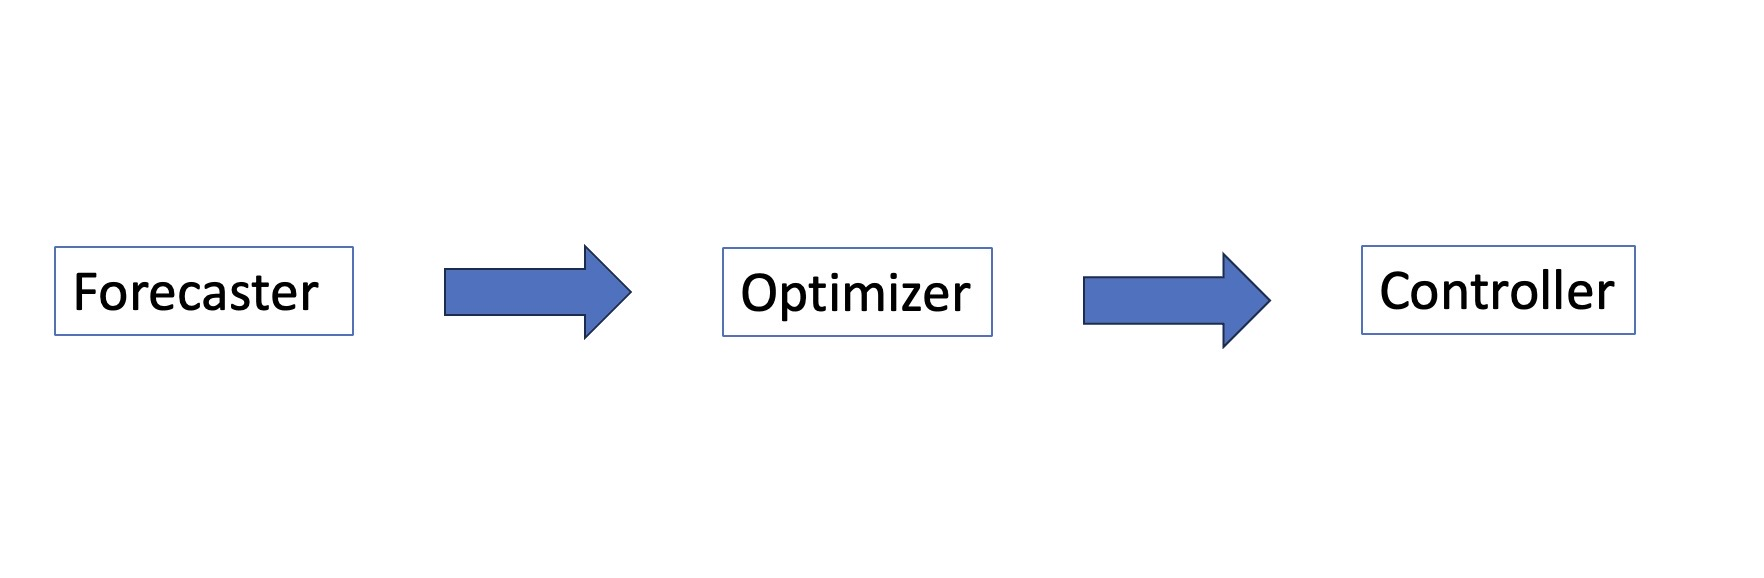
\includegraphics[width=\textwidth]{Figures/06Design/control_overview.jpg}
    \caption[Control system components]{Control system components}
    \label{fig:control_syst}
\end{figure}


\section{Load analysis}

Chiwoza is, as shown in figure \ref{fig:system_topology}, solely powered by a hybrid source consisting of a battery and PV-module. As solar power is an intermittent and \textit{non-dispatchable} resource, the only control levers are the power to and from the battery and the enabling/disabling of loads. To control a system by adjusting the load is known as \textit{demand-side-management}(DSM). For a DSM-control system to be effective, a thorough and accurate understanding of the connected loads is necessary. This is gained through load analysis. There are 3 main goals to be achieved from this process:
\begin{enumerate}
    \item \textbf{Understand consumption pattern}    - The total consumption varies both in how much power is demanded, and when it is demanded. This is also true on the disaggregated level for the consumption for each load. This creates a consumption pattern across time. When attempting to control the consumption, the goal is to predict the pattern into the future. This will is the subject of the next section \ref{seq:load_forecasting} on load forecasting. A prerequisite for the work in that section is an understanding of the historical consumption pattern.
    \item \textbf{Understand load value}    -   As loads vary in their purpose, the end users will value the available loads differently. This valuation is unlikely to be static but will vary based on circumstances such as the time of day. The control system will prioritize certain loads over others. This prioritization should be partly based on how the end-users value the loads present at the site. The information about valuation is gained through a user survey described in section \ref{seq:user_survey}.
    \item \textbf{Classifying types of loads}   -   Loads also differ in other aspects, such as the flexibility of demand. Certain loads need to satisfy an immediate goal, while others are more flexible in when demand can be met. Understanding this difference between the loads is fundamental for identifying the available control options. This work is done in section \ref{seq:load_classification}.
\end{enumerate}

For this thesis, the load analysis was performed through the gathering of transmitted data and user queries. The available data from the monitoring system detailed in subsection \ref{seq:data_collection}. The most important being the time-series showing the disaggregated-by-meter and total consumption.\\

\subsection{Statistical analysis}

The statistical load analysis attempts to draw conclusion based on historic data. Starting out by considering the total daily consumption, plotted from October 23rd to December 23rd 2023 in figure \ref{fig:tot_con_daily_chiwoza_20231023-1223}  seems to vary around a mean. At the the 20th of December, there seems to be a significant drop in consumption. This could reflect an actual lower consumption, a problem with the data or a failure of the system.\\ 

It is also possible to examine consumption at a higher time-resolution, down to the hourly level. Figure \ref{fig:tot_con48_chiwoza_202310} shows the consumption in October 2023 plotted as successive 48-hour periods. Each gray line represents a 48-hour period. These are mostly centred around the average, shown in blue. It is clear that for total consumption, the variance within a day is much larger than the variance between days. There are certain spikes indicating a sudden large, but short-lasting consumption during the daytime. The section \ref{seq:current_syst} on current control measures states that certain high power loads are set to run only at specific time intervals during the day. This pattern is likely a cause of that.\\

\begin{figure}
    \centering
    \includegraphics[width=\textwidth]{Figures/06Design/tot_con_daily_chiwoza_20231023-1223.png}
    \caption[Daily consumption Chiwoza 20231023-1223]{The total daily consumption of Chiwoza from October 23rd to December 23rd 2023. Included with the 5 day average. Weekends are shaded in grey.}
    \label{fig:tot_con_daily_chiwoza_20231023-1223}
\end{figure}

\begin{figure}
    \centering
    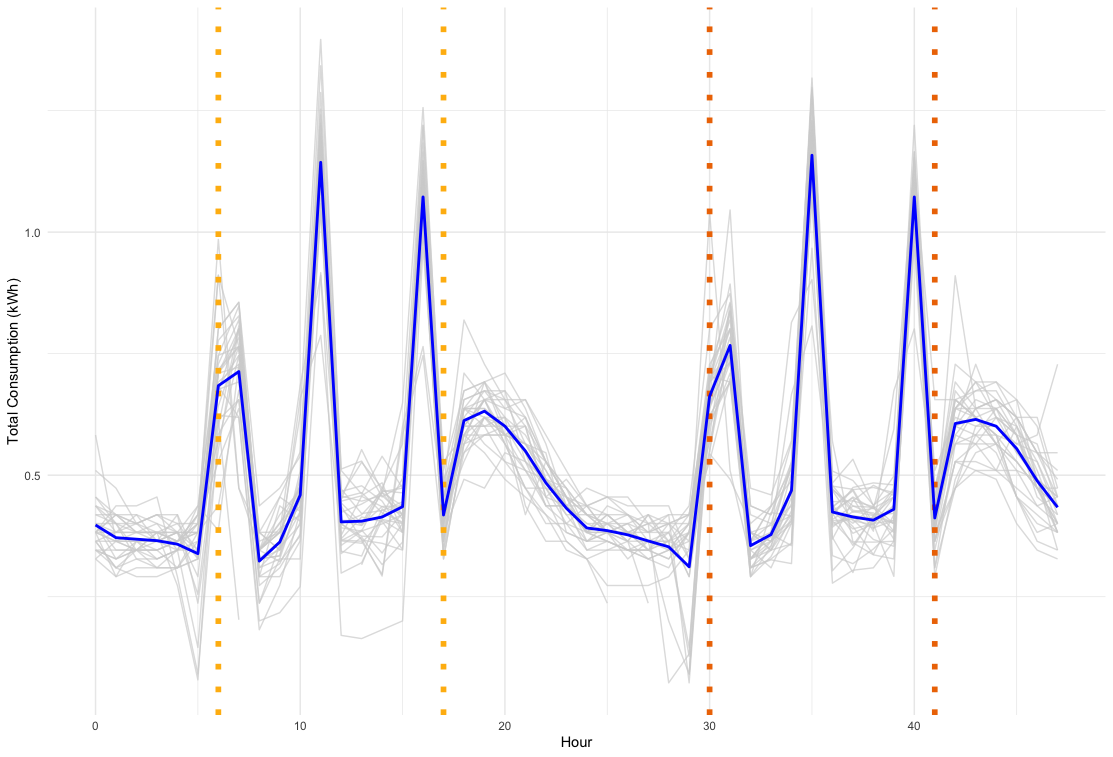
\includegraphics[width=\textwidth]{Figures/06Design/tot_con48_chiwoza_202310.png}
    \caption[Consumption Chiwoza October successive 48h-periods]{The total consumption of Chiwoza for successive 48-hour periods starting at midnight over the month of October 2023. The average across the month is highlighted in blue, and the start and end of normal daylight time is indicated by the doted lines for the two days respectively. The spikes in the pattern is due to time-regulated usage of a heavy use water pump.}
    \label{fig:tot_con48_chiwoza_202310}
\end{figure}

The total consumption of a site may be split into the consumption measured by the meters mounted at the various circuits. This yields a disaggregated view of the consumption based on the specific usage. As outlined in section \ref{seq:data_collection}, this is the highest level of resolution on which to analyse historical consumption data. In figure \ref{fig:con_disagg_chiwoza_20230603-05} the consumption of Chiwoza over a 48 hour period in June 2023 is disaggregated based on meter. This plot supports the proposal in the previous paragraph, that the spikes in consumption were caused by time controlled high-powered loads. The fact that these loads are already controlled, suggests that these are flexible. This means that their past pattern is less interesting, because the pattern can be adjusted as need be. For the other loads, the pattern is important as it is inflexible. Neglecting the flexible loads, the consumption seems to be dominated by the Medical Light and Staff Socket consumption. For the Medical Light not surprisingly there is an increase in consumption during nighttime. This creates a repeating pattern each day. Repeating patterns over a period is known as periodicity, which is a key characteristic to identify for a load. We can be confident that most loads will have periodicity within a day. In addition, some loads might exhibit patterns between days. Identifying these will greatly improve the foundation for forecasting.\\ 

\begin{figure}[h]
    \centering
    \includegraphics[width=\textwidth]{Figures/06Design/con_disagg_chiwoza_20230603-05.png}
    \caption[Disaggregated Consumption Chiwoza 20230603-05]{The disaggregated consumption of Chiwoza over a 48 hour period starting from midnight 2023-06-03. As opposed to the rest of the thesis, the date was selected so far back because afterwards a communication problem with the meter on the water heater occurred. In later analysis, loads such as Staff Sockets 1 and 2 have recorded no consumption. }
    \label{fig:con_disagg_chiwoza_20230603-05}
\end{figure}

\subsubsection{Patterns between days}\label{seq:periodicity}

A natural first assumption is that some loads will show a difference in consumption between workdays and weekends. Despite being a health site, where medical emergencies might suddenly require attention, Chiwoza follows a regular Malawian workweek from Monday to Friday. Looking first at the total consumption, the weekends are shaded grey in figure \ref{fig:tot_con_daily_chiwoza_20231023-1223} showing the total consumption. From the plot alone, there is no clear difference between weekdays and weekends for the total consumption. The ACF can also be used to indicate a pattern. If the consumption was largely different between weekdays and weekends, this would have shown up in the ACF as high values at lags corresponding to the current day of the week. The ACF across the entire period, shown in \ref{fig:con_acf_day_chiwoza_201023-1223}, shows no such pattern. There are no public holidays in Malawi during this period either, so that is no factor. The analysis does therefore not show enough to support a claim that the day of the week influences the total consumption significantly. However, there might be such a pattern for certain loads. \\

\begin{figure}[h]
    \centering
    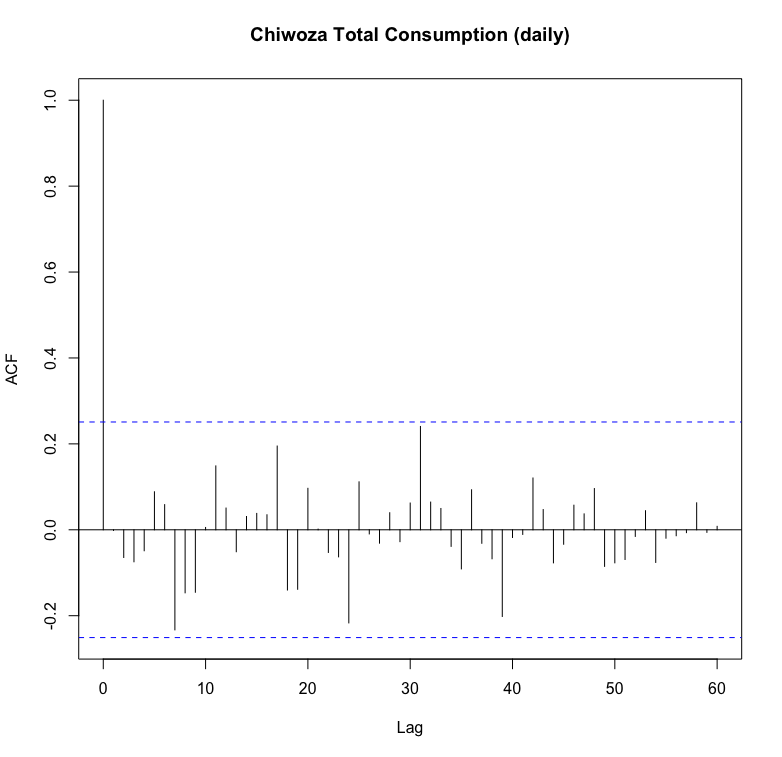
\includegraphics[width=\textwidth]{Figures/06Design/con_acf_day_chiwoza_201023-1223.png}
    \caption[ACF Daily consumption Chiwoza 20231023-1223]{ACF of the total daily consumption at Chiwoza. Lags represent the amount of days back from December 23rd 2023.}
    \label{fig:con_acf_day_chiwoza_201023-1223}
\end{figure}

The same kind of analysis as performed above can be done on individual loads. The medical light consumption, shown in figure \ref{fig:con_chiwoza_med_light_20231023-1223} has no clear pattern between days. Neither does staff consumption, as seen in figure \ref{fig:con_chiwoza_staff_20231023-1223}. The two loads Medical Sockets and Guardian Shelter Socket, shown in \autoref{fig:con_chiwoza_med_socket_20231023-1223} and \autoref{fig:con_chiwoza_guard_socket_20231023-1223} respectively does however indicate some difference in consumption between weekdays and weekends. The pattern at the Guardian Shelter Socket especially, shows a clear difference, with its consumption happening almost exclusively on weekdays. The ACF across the period for the Guardian shelter supports this as, shown in figure \ref{fig:con_acf_chiwoza_guard_socket_20231023-1223}, the lag representing 7 days back from December 23rd, a Saturday, is significant. The ACF for the consumption from the Medical Socket, in figure \ref{fig:con_acf_chiwoza_med_socket_20231023-1223} is less clear, with no significant daily lags. This indicates that the difference in consumption between weekdays and weekends is larger for the Sockets at the Guardian Shelter than for the Medical Building. There is also not the same pattern for the light consumption at the guardian shelter, seen in \ref{fig:con_ts_chiwoza_guard_light_202311}, suggesting that the lights are on independently of the day of the week. The last load, the fence light shown in figure \ref{fig:con_chiwoza_fence_light_20231023-1223}, have no clear pattern either. The consumption here is also so small, averaging to less than 25Wh a day, so small deviations have a large effect. \\

\begin{figure}[]
    \centering
    \includegraphics[width=\textwidth]{Figures/06Design/con_chiwoza_med_light_20231023-1223.png}
    \caption[Medical Light consumption Chiwoza 20231023-1223]{Light consumption in the medical buildings at Chiwoza from October 23rd to December 23rd 2023. 5-day average as a dotted line. Weekends are shaded in grey.}
    \label{fig:con_chiwoza_med_light_20231023-1223}
\end{figure}

\begin{figure}[]
    \centering
    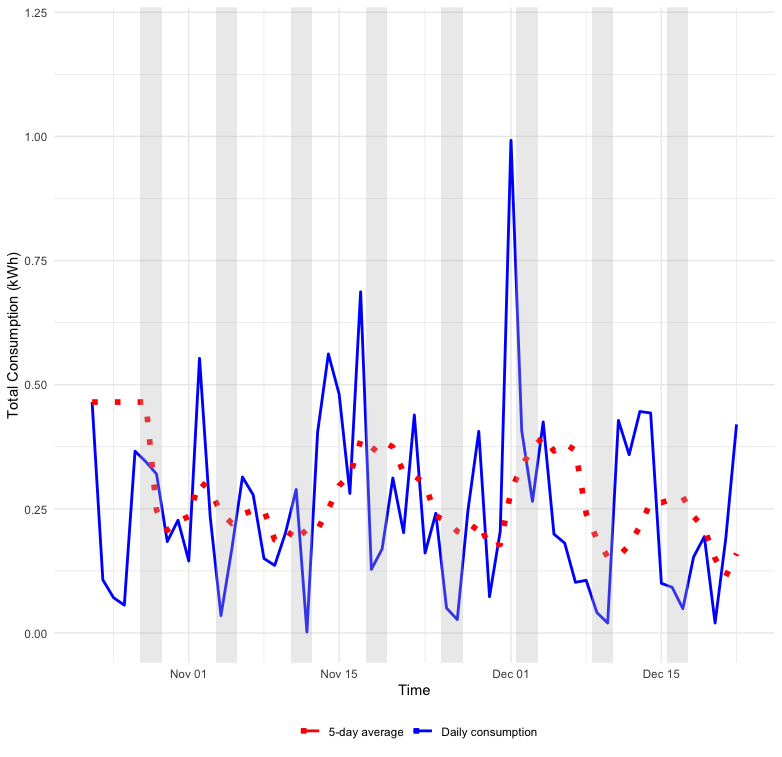
\includegraphics[width=\textwidth]{Figures/06Design/con_chiwoza_med_socket_20231023-1223.png}
    \caption[Medical Socket consumption Chiwoza 20231023-1223]{Consumption from the sockets at the medical building at Chiwoza from October 23rd to December 23rd 2023. 5-day average as a dotted line. Weekends are shaded in grey.}
    \label{fig:con_chiwoza_med_socket_20231023-1223}
\end{figure}

\begin{figure}[]
    \centering
    \includegraphics[width=\textwidth]{Figures/06Design/con_chiwoza_guard_socket_20231023-1223.png}
    \caption[Guardina Shelter Socket consumption Chiwoza 20231023-1223]{Consumption from the sockets at the Guardian Shelter at Chiwoza from October 23rd to December 23rd 2023. 5-day average as a dotted line. Weekends are shaded in grey.}
    \label{fig:con_chiwoza_guard_socket_20231023-1223}
\end{figure}

\begin{figure}[]
    \centering
    \includegraphics[width=\textwidth]{Figures/06Design/con_chiwoza_guard_light_20231023-1223.png}
    \caption[Guardian Shelter Light consumption Chiwoza 20231023-1223]{Consumption from the Lights at the Guardian Shelter at Chiwoza from October 23rd to December 23rd 2023. 5-day average as a dotted line. Weekends are shaded in grey.}
    \label{fig:con_chiwoza_guard_light_20231023-1223}
\end{figure}

\begin{figure}[]
\centering
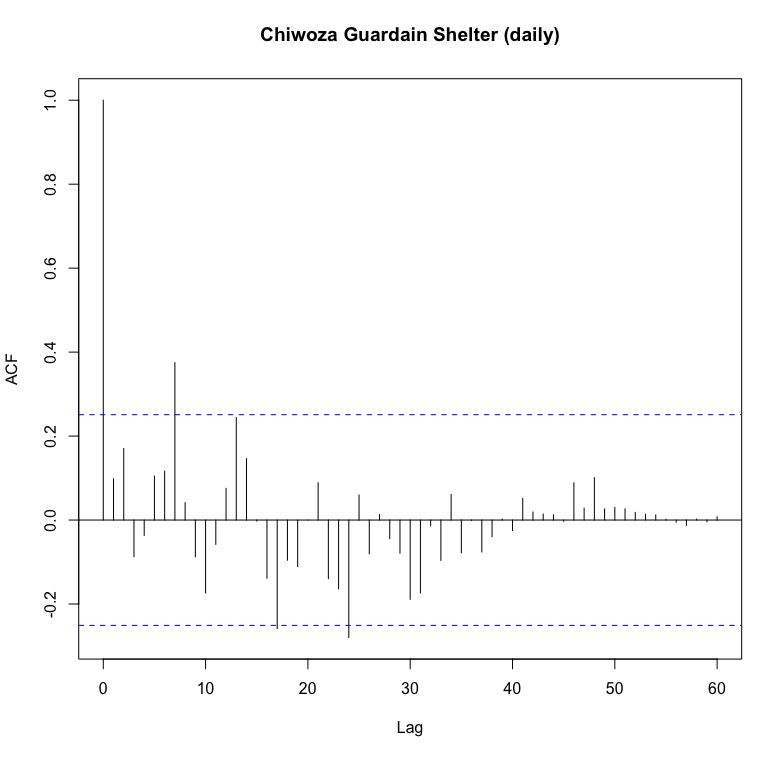
\includegraphics[width=\textwidth]{Figures/06Design/con_acf_chiwoza_guard_socket_20231023-1223.png}
\caption[ACF Guardian shelter socket consumption Chiwoza 20231023-1223]{Auto correlation of consumption measured from the sockets at the Guardian Shelter at Chiwoza between October 23rd to December 23rd 2023. Blue dotted lines represent a 95\% confidence interval.}
\label{fig:con_acf_chiwoza_guard_socket_20231023-1223}
\end{figure}

\begin{figure}[]
\centering
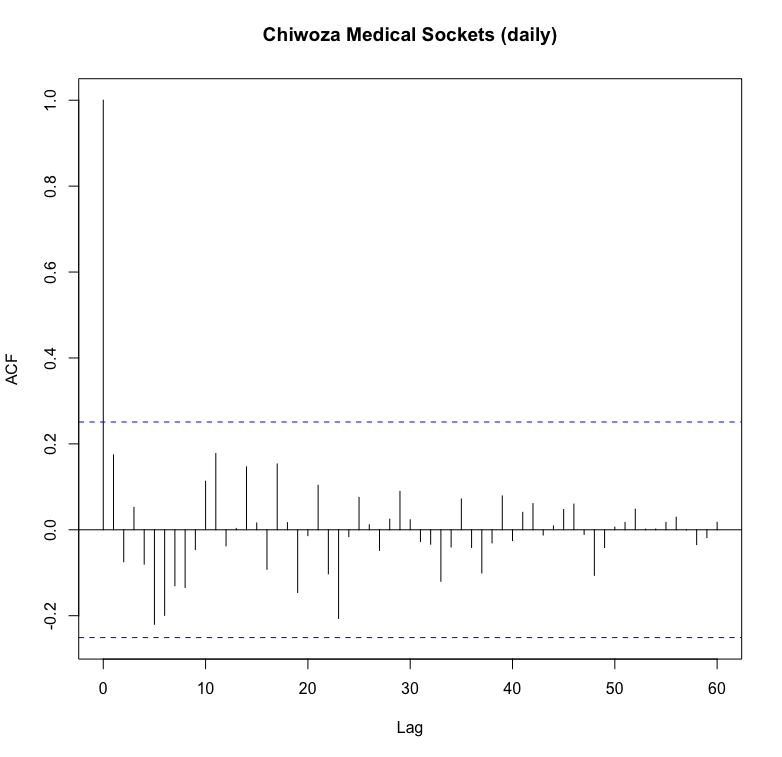
\includegraphics[width=\textwidth]{Figures/06Design/con_acf_chiwoza_med_socket_20231023-1223.png}
\caption[ACF Medical Socket consumption Chiwoza 20231023-1223]{Auto correlation of consumption measured from the sockets at the Medical Building at Chiwoza between October 23rd to December 23rd 2023. Blue dotted lines represent a 95\% confidence interval.}
\label{fig:con_acf_chiwoza_med_socket_20231023-1223}
\end{figure}

\begin{figure}[]
    \centering
    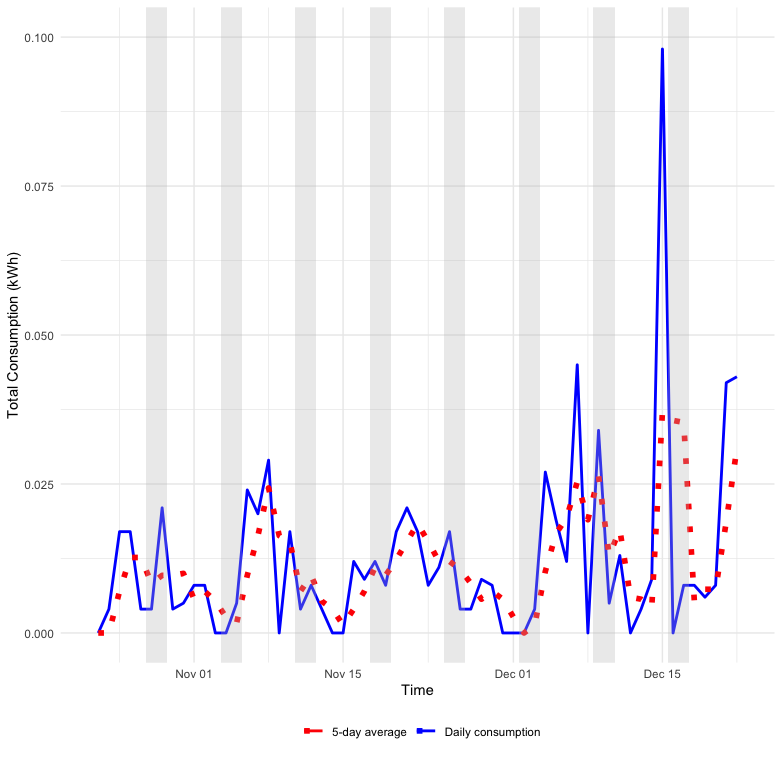
\includegraphics[width=\textwidth]{Figures/06Design/con_chiwoza_fence_light_20231023-1223.png}
    \caption[Fence Light consumption Chiwoza 20231023-1223]{Fence light consumption at Chiwoza from October 23rd to December 23rd 2023. 5-day average as a dotted line. Weekends are shaded in grey.}
    \label{fig:con_chiwoza_fence_light_20231023-1223}
\end{figure}

\begin{figure}[]
  \centering
  \begin{minipage}{0.7\textwidth} % Adjust the width as needed
    \centering
    \includegraphics[width=\linewidth]{Figures/06Design/con_chiwoza_staff_light_20231023-1223.png}
    \caption[Staff Light consumption Chiwoza 20231023-1223]{Daily light consumption in the staff buildings at Chiwoza between October 23rd to December 23rd 2023. Weekends are shaded in grey.}
    \label{fig:con_chiwoza_staff_light_20231023-1223}
  \end{minipage}

  \vspace{0.5cm} % Add vertical space between the subfigures

  \begin{minipage}{0.7\textwidth} % Adjust the width as needed
    \centering
    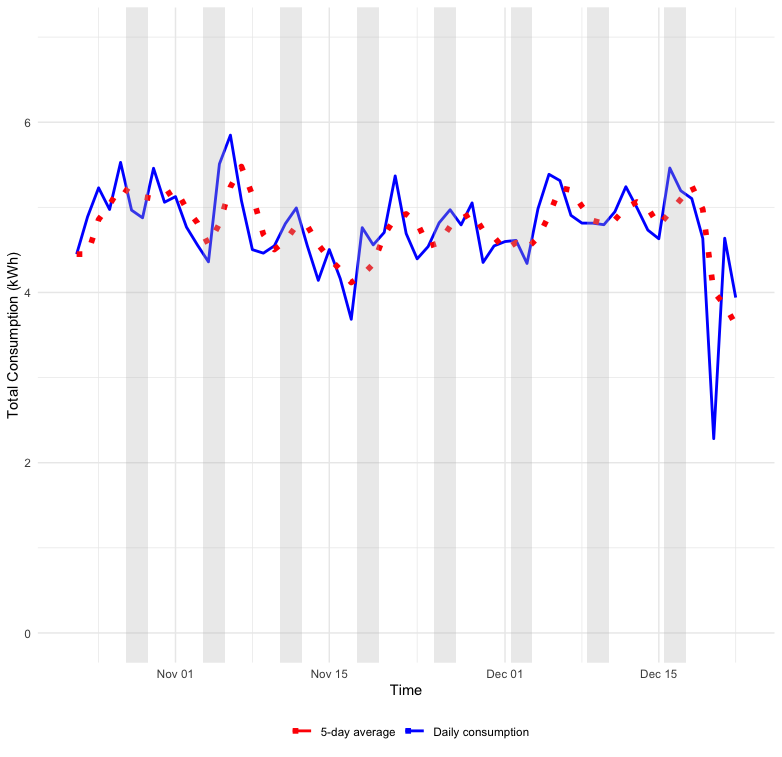
\includegraphics[width=\linewidth]{Figures/06Design/con_chiwoza_staff_socket_20231023-1223.png}
    \caption[Staff Socket consumption Chiwoza 20231023-1223]{Daily consumption measured from the sockets at the staff buildings at Chiwoza between October 23rd to December 23rd 2023. Weekends are shaded in grey.}
    \label{fig:con_chiwoza_staff_socket_20231023-1223}
  \end{minipage}

  \caption[Staff consumption Chiwoza 20231023-1223]{Daily consumption at staff buildings in November 2023.}
  \label{fig:con_chiwoza_staff_20231023-1223}
\end{figure}

In summary, the load analysis has identified that apart from the flexible loads, the consumption is dominated by staff and medical usage. These have a clear periodic pattern within a day, but for most of them, no obvious between days. The two exceptions, The Medical Sockets and especially the Guardian Shelter Socket, have a clear enough difference in consumption between the weekdays and weekends to warrant extra consideration for the forecasting.

\subsection{User survey}\label{seq:user_survey}
A user survey was developed for this thesis in collaboration with DCP. It was performed through phone calls by a local representative to staff members to staff members at the site. A total of 19 sites participated in the survey, all listed in \ref{tab:us_participants}. These vary in size, purpose and location. The goal of the survey was:
\begin{itemize}
    \item \textit{Map out connected loads}  - Finding which loads are connected to the various sites.
    \item \textit{Discover load prioritization} - Examining how the users value and use the different loads at various times during the day.
    \item \textit{Determining the acceptability for control}    - Determining how able the users are to understand and accept an automatic control system. 
\end{itemize}

In this section, the results relating to loads are discussed. The full results from the questionnaire are included in appendix \ref{appendix:user_survey}. \\

Table \ref{tab:connected_loads} shows the loads reported to be currently connected at the queried sites. When asked to prioritize amongst loads during daytime and nighttime, figure \ref{fig:user_survey_load_daytime_1st&2nd_priority} and \ref{fig:user_survey_load_nighttime_1st&2nd_priority} shows a clear pattern. The users appear on average to value loads related to the purpose of the site higher than loads related to the leisure of the staff members. This pattern is stronger during the daytime, but even during the night, the first priority is clearly to keep the lights on at the facilities. This is supported by the results in section \ref{seq:forced_choice}, where most respondents answer that they are willing to forgo some days of staff consumption to ensure the availability of critical loads.

\begin{figure}[]
  \centering

  % First Subfigure
  \begin{subfigure}{\textwidth}
    \centering
    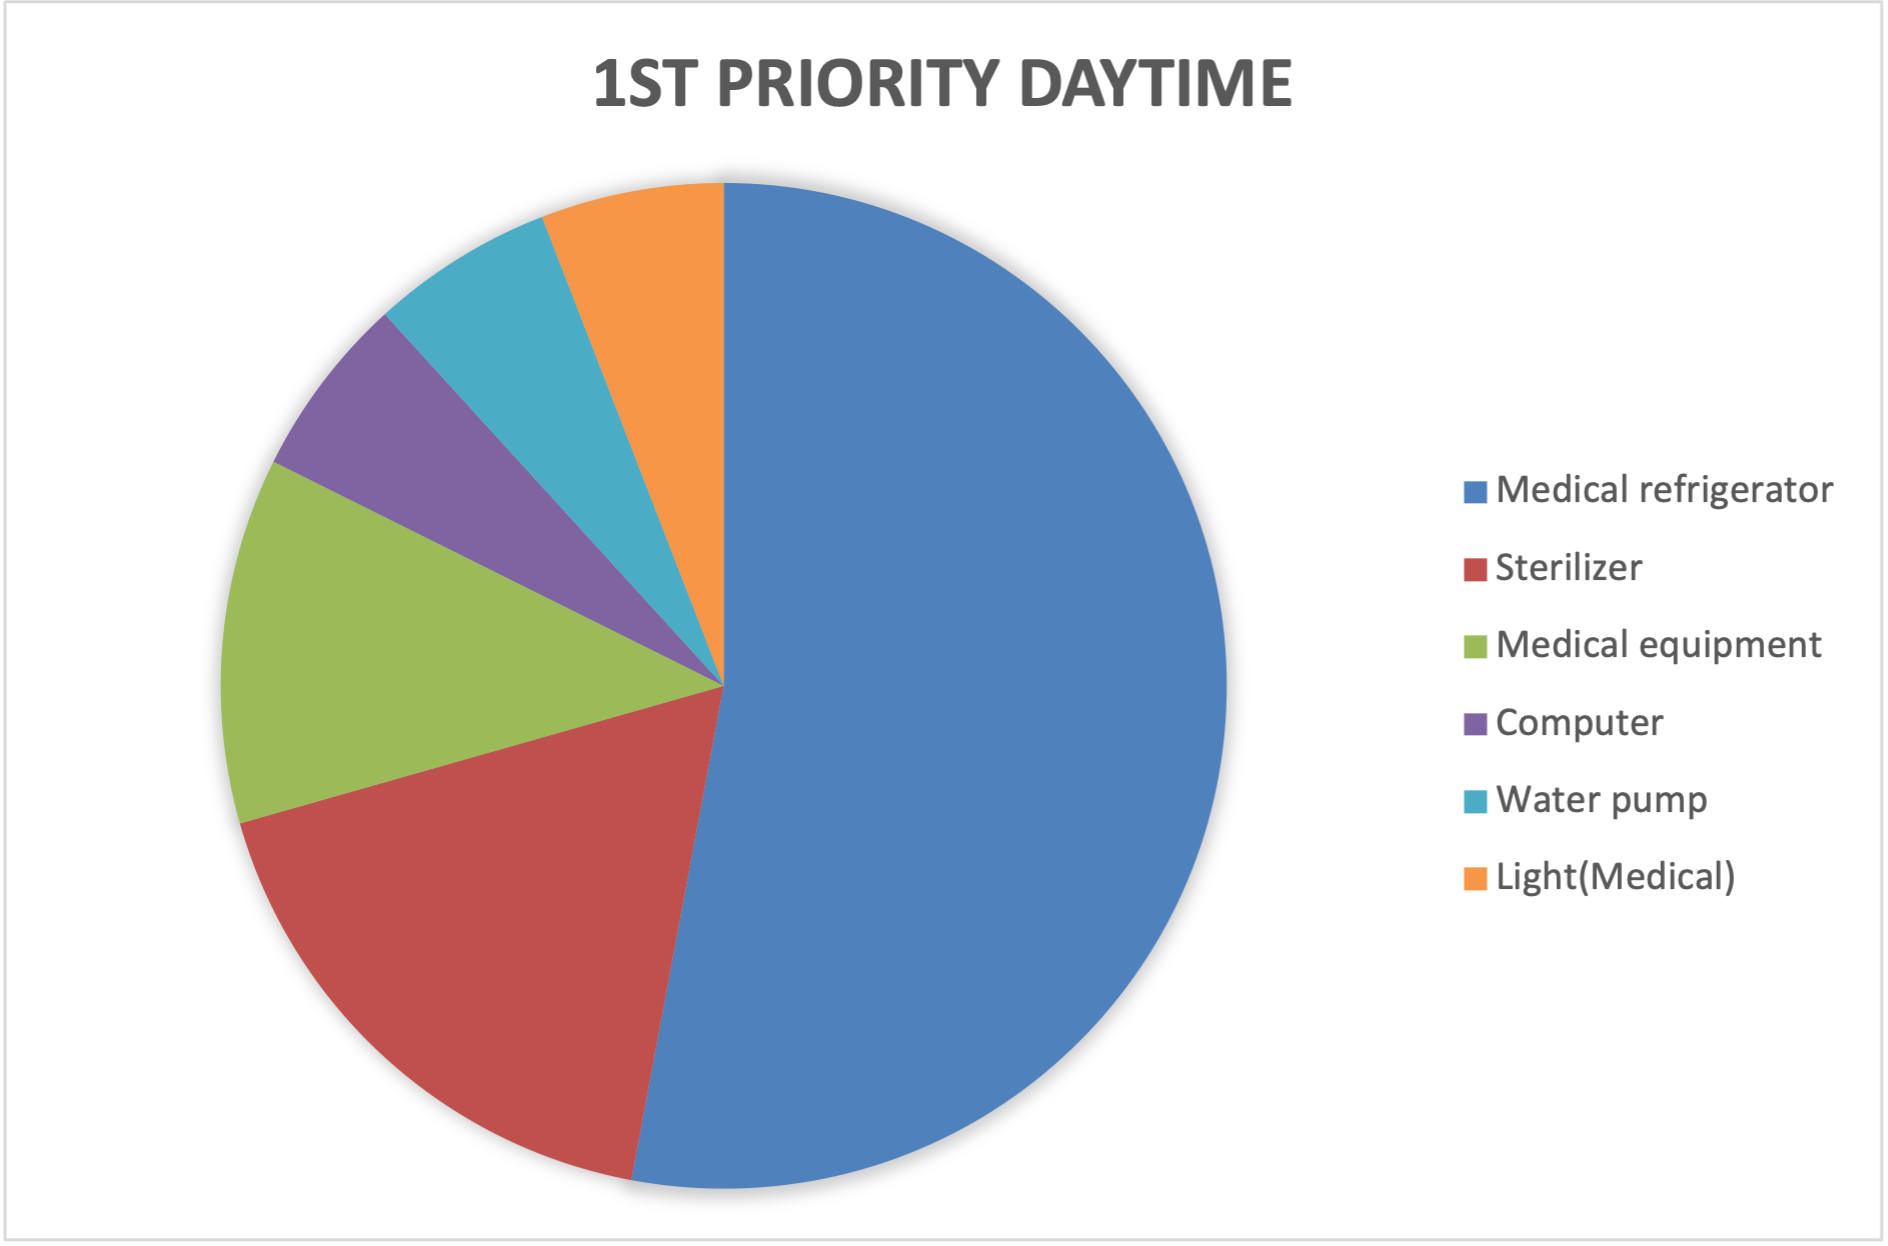
\includegraphics[width=\linewidth]{Figures/06Design/user_survey_load_daytime_1st_priority.png}
    \caption[User survey: Daytime 1st priority]{Reported 1st priority amongst loads during daytime}
    \label{fig:user_survey_load_daytime_1st_priority}
  \end{subfigure}

  % Add some vertical space between the subfigures
  \vspace{0.5cm}

  % Second Subfigure
  \begin{subfigure}{\textwidth}
    \centering
    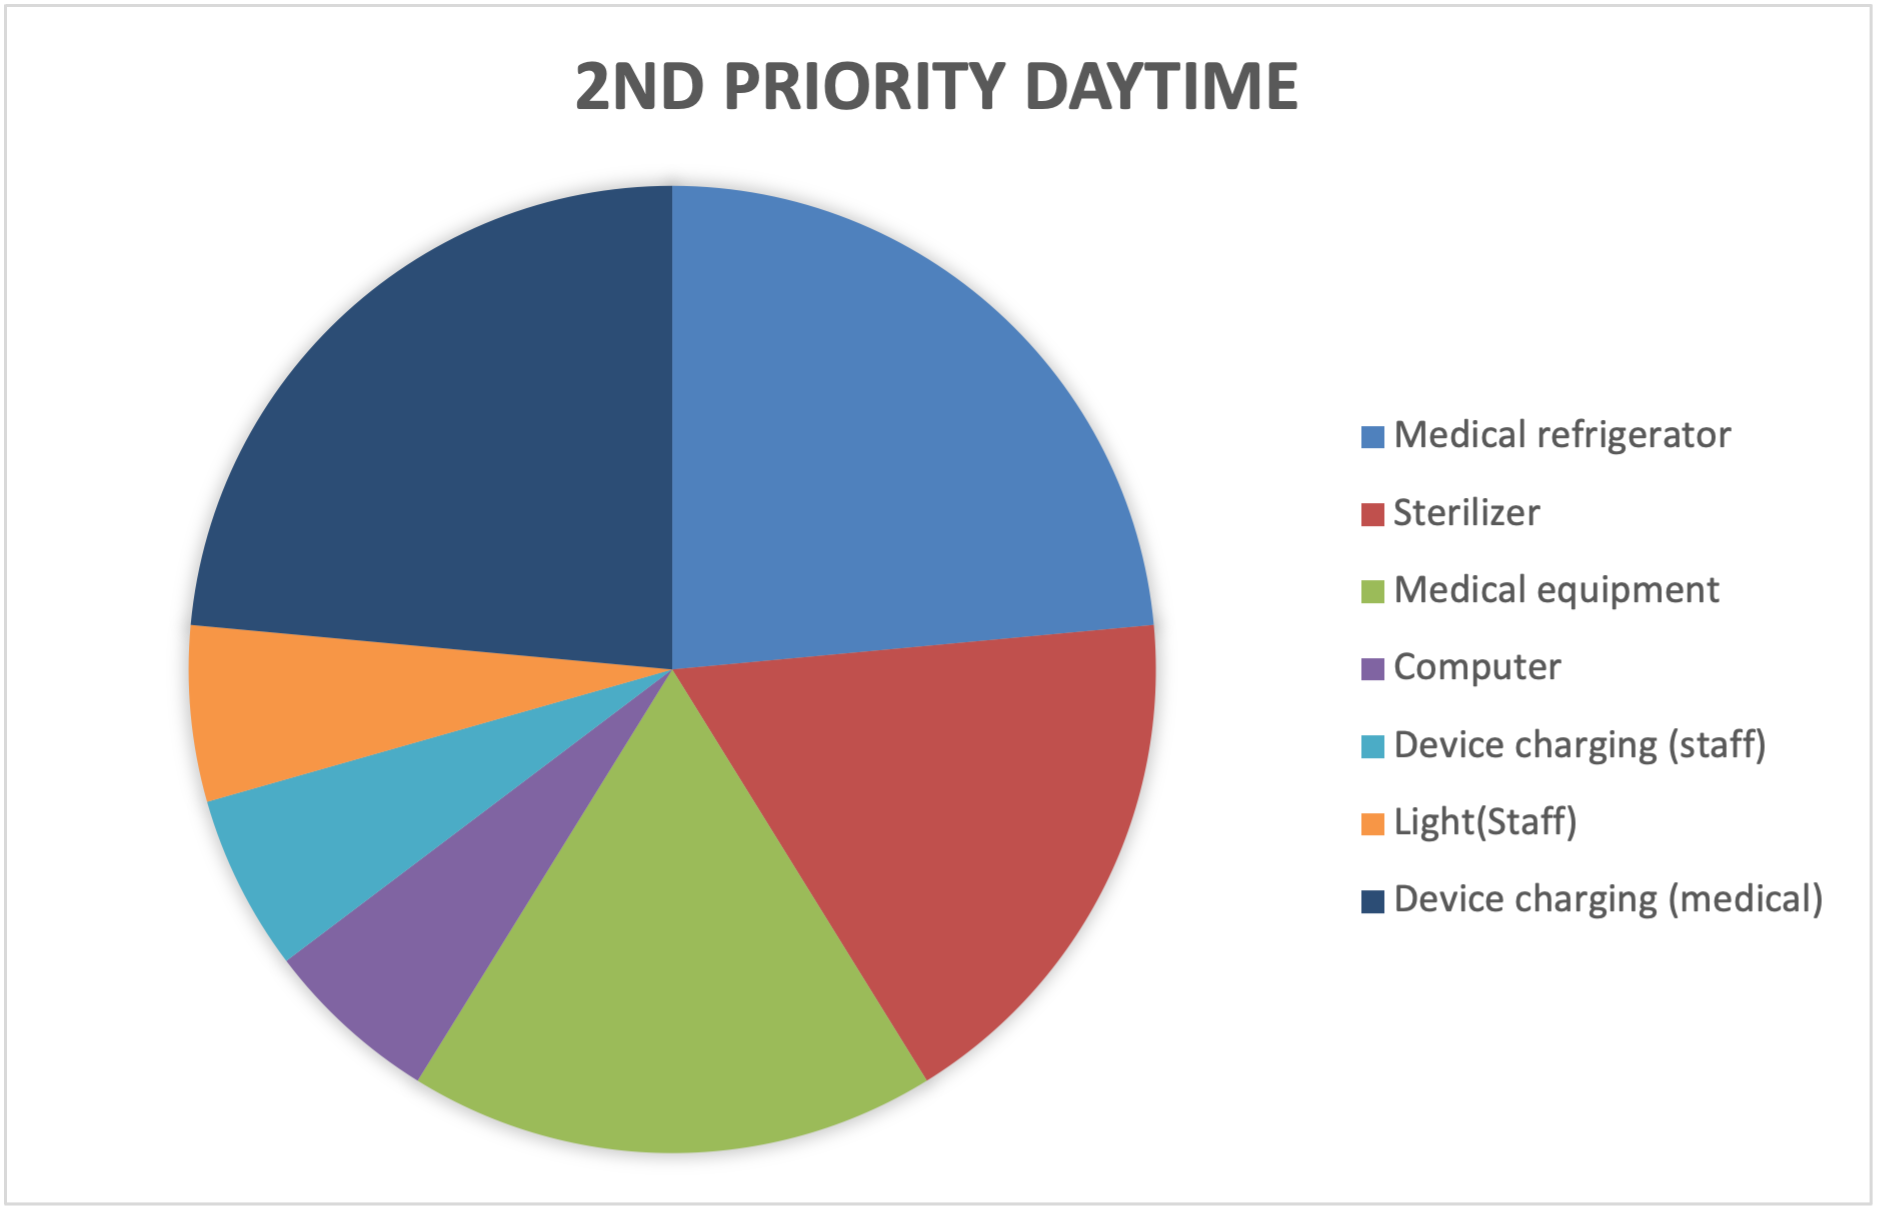
\includegraphics[width=\linewidth]{Figures/06Design/user_survey_load_daytime_2nd_priority.png}
    \caption[User survey: Daytime 2nd priority]{Reported 2nd priority amongst loads during daytime.}
    \label{fig:user_survey_load_daytime_2nd_priority}
  \end{subfigure}

  \caption[User survey: Daytime priority]{Reported 1st and 2nd priority amongst loads during daytime.}
  \label{fig:user_survey_load_daytime_1st&2nd_priority}
\end{figure}


\begin{figure}[]
  \centering

  % First Subfigure
  \begin{subfigure}{\textwidth}
    \centering
    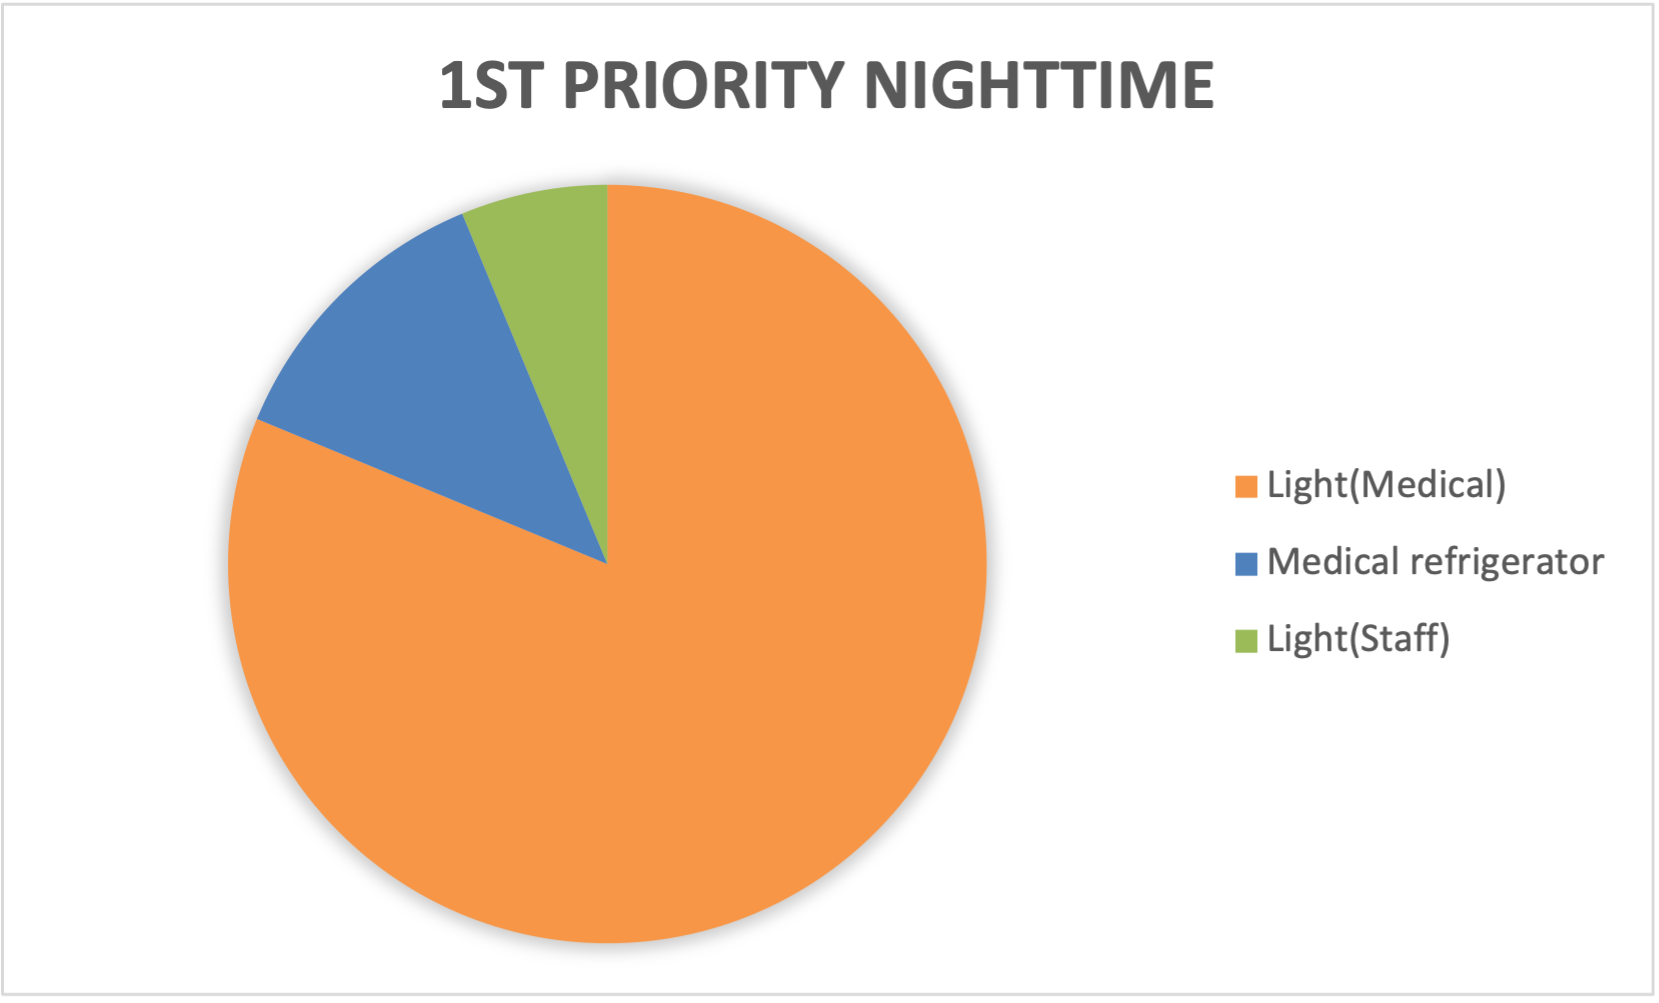
\includegraphics[width=\linewidth]{Figures/06Design/user_survey_load_nighttime_1st_priority.png}
    \caption[User survey: Nighttime 1st priority]{Reported 1st priority amongst loads during nighttime}
    \label{fig:user_survey_load_nighttime_1st_priority}
  \end{subfigure}

  % Add some vertical space between the subfigures
  \vspace{0.5cm}

  % Second Subfigure
  \begin{subfigure}{\textwidth}
    \centering
    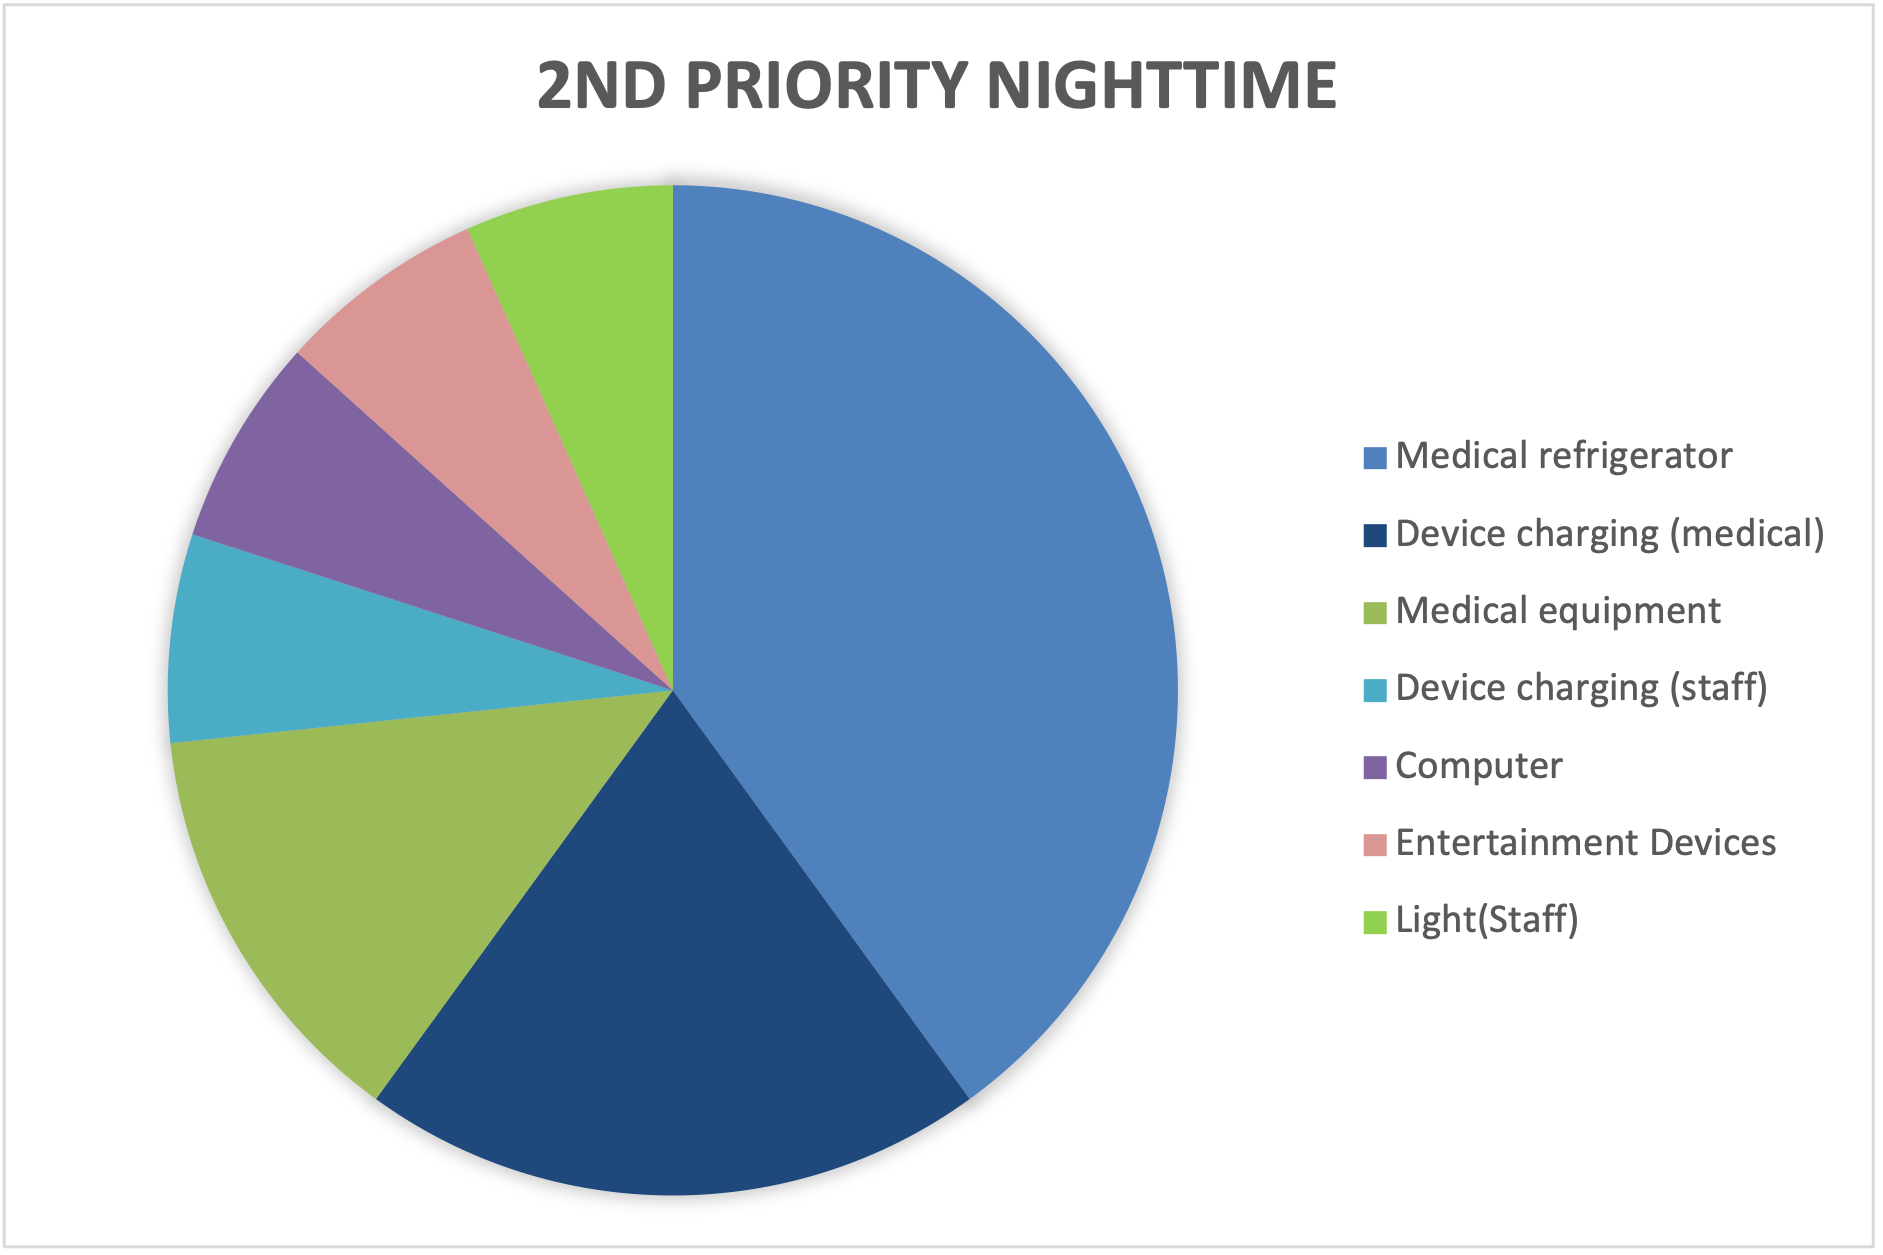
\includegraphics[width=\linewidth]{Figures/06Design/user_survey_load_nighttime_2nd_priority.png}
    \caption[User survey: Nighttime 2nd priority]{Reported 2nd priority amongst loads during nighttime.}
    \label{fig:user_survey_load_nighttime_2nd_priority}
  \end{subfigure}

  \caption[User survey: Nighttime priority]{Reported 1st and 2nd priority amongst loads during nighttime.}
  \label{fig:user_survey_load_nighttime_1st&2nd_priority}
\end{figure}



\subsection{Load classification}\label{seq:load_classification}
As seen in the previous section, there are several different kinds of loads installed at the various sites. These vary in their importance for the operation at the site, their electrical characteristics and the characteristics important for controlling the system. Using the classification from \cite{Philipo2022-rx}, the classifying control characteristics are 
\begin{itemize}
    \item \textit{Deferable} -   The ability to defer a load to a different time without a penalty. This is only possible if a demand does not need to be instantaneously met. For instance, if the demand for light, TV or Microscope is not met immediately when demanded, it is noticed by the user. Other loads, such as the water pump, do not have this requirement. Although the demand for water is non-deferable, the pump itself supplies water to a tank, hence as long as the tank has water there is no penalty for deferring the running of the water pump. 
    \item \textit{Dimable}  -   A dimable load can run on various power levels
    \item \textit{Interuptable} -   An interruptable load can be interrupted after being started without any additional penalty. 
\end{itemize}

In addition to these, loads are also assigned a priority, which translates into a penalty for not being allowed to run when demanded. As seen from the user survey, the end-users value different loads higher at different times. The priority is therefore not static, but may change during the day. The various loads found to be connected during the user survey are classified in table \ref{tab:load_control} \\

\begin{table}[]
    \centering
    \small
    \begin{tabular}{|>{\raggedright\arraybackslash}p{4cm}|p{1.5cm}|p{1.5cm}|p{2cm}|}
         Load & Deferable & Dimable & Interuptable \\
         \hline
         Lights (Medical/School) & NO & NO & NO\\
         Phone/Laptop Charging (Medical) & YES & YES & YES\\
         Oxygen Concentrator & NO & NO & NO\\
         HIV diagnosis equipment & NO & NO & NO\\
         Sterilizer & NO & NO & YES\\
         Microscope & NO & NO & NO\\
         Refrigerator (Medical) & NO & NO & NO\\
         \hline
         Light (Staff) & NO & NO & NO\\
         Phone/Laptop Charging (Staff) & YES & YES & YES\\
         Entertainment & NO & NO & NO\\
         Refrigerator (Staff) & NO & NO & NO\\                  
         Cooking appliances & NO & NO & NO\\
         \hline
         Water pump & YES & YES & YES\\
         Water heater & YES & YES & YES\\
         \hline
    \end{tabular}
    \caption[Connected loads control attributes]{Loads connected to the systems with their control attributes}
    \label{tab:load_control}
\end{table}

As mentioned in section \ref{seq:data_collection}, loads are not measured individually, but based on the circuit they are connected to. While there could potentially be a method of identifying a specific load through the consumption measured from the circuit, this has not been attempted in this thesis. As a result, the resolution of classification decreases to the circuit level. Mapping the control characteristics from \autoref{tab:load_control} to the circuits in \autoref{tab:loads_chiwoza} yields the circuit level control characteristics in \autoref{tab:circuit_control}. For the rest of the design, this will be the level of resolution, the term load is therefore broadened to include all individual loads connected to a circuit. 

\begin{table}[]
    \centering
    \small
    \begin{tabular}{|>{\raggedright\arraybackslash}p{4cm}|p{1.5cm}|p{1.5cm}|p{2cm}|}
         Circuit & Deferable & Dimable & Interuptable \\
         \hline
         Medical Light & NO & NO & NO\\
         Medical Socket & NO & NO & NO\\
         Staff Light 1-3 & NO & NO & NO\\
         Staff Socket 3 & NO & NO & NO\\
         Guardian Shelter Light & NO & NO & NO\\
         Guardian Shelter Socket & NO & NO & NO\\
         Fence Light & NO & NO & NO\\
         \hline
         Water pump & YES & YES & YES\\
         Water heater & YES & YES & YES\\
         \hline
         Solar Maize Mill & YES & YES & YES\\
         Rental Batteries & YES & YES & YES\\
         \hline
    \end{tabular}
    \caption[Circuits control attributes]{Circuits connected to the systems with their control attributes}
    \label{tab:circuit_control}
\end{table}

\subsubsection{Flexible Loads definition and analysis}\label{seq:flex_loads}
From a control perspective, the last 4 loads of table \ref{tab:circuit_control} are the most interesting. Because their demand is flexible, they offer the prime control option to be utilized. These \textit{flexible loads} are characterized by the following:
\begin{itemize}
    \item \textit{Energy Demand}    -   Within a day, these loads demand to be run enough to perform some task. For the water pump, this will be to fill the tank with enough water to satisfy a day's demand, if the tank is large enough to support that. For the water heater, this will be to heat enough water to last some hours in the future. The key is that the energy demand does not have to be satisfied immediately, but within some time window.
    \item \textit{Power Demand}     -   If the flexible load is running, it requires a certain amount of power to be able to run. This is the power demand. 
    \item \textit{Operation Window} -   The operation window specifies within which time window a flexible load can run. For instance, the solar Maize mill should be running during the day, because that is when the farmers can deliver and collect their goods.   
\end{itemize}

As these loads are more clearly defined, the values can be found from datasheets\cite{wp_documentation}\cite{water_heater}\cite{maize_mill}. The water pump at Chiwoza is a \textit{SQF5-70} from Grundfos. These are powered by  a \textit{universal motor}. A universal motor can be controlled by regulating the current supplied to the motor. Figure \ref{fig:wp_power_flow_curve} from the datasheet provided by the manufacturer relates the power to water depth and flow. Similarly, the figures for the power rating for the other flexible loads are found in the datasheets and included in \ref{tab:flexible_loads_characteristics}. The daily energy demand for the water pump and heater is determined as the average historical daily consumption. For the two loads that have not been connected, the maize mill and rental batteries, their daily demand is determined through internal economic calculations by DCP on how often they need to run to be economically feasible for DCP to install at the sites.\\

\begin{figure}[]
    \centering
    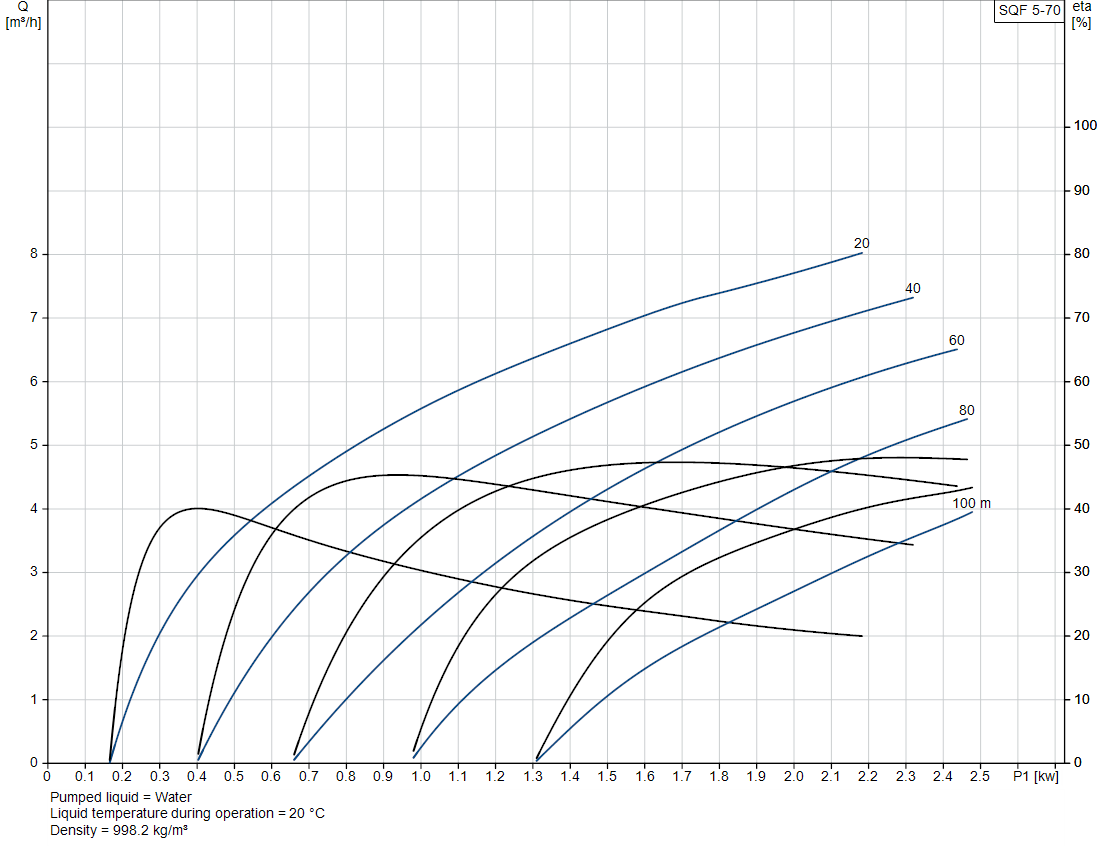
\includegraphics[width=\textwidth]{Figures/06Design/wp_sqf25-2_power_curve.png}
    \caption[Water pump power/flow-curve]{Power-flow curve for the water pump installed at Chiwoza. Along the y-axis is the flow measured in [m2/h] while along the x-axis is the power in kW. The blue lines show the depth of the well.}
    \label{fig:wp_power_flow_curve}
\end{figure}

\begin{table}[]
    \centering
    \begin{tabular}{c|c|c|c|c}
       Load  & Min Power (W) & Max Power (W)& Energy Demand Daily (Wh) \\
       \hline
       Water Pump  & 400 & 1100 & 2750 \\
       Water Heater  & 200 & 350 & 1400 \\
       Rental Batteries  & 10.8 & 270 & 540 \\
       Maize Mill  & 800 & 3000 & 9750 \\
    \end{tabular}
    \caption[Flexible Loads energy characteristics]{Flexible Loads energy characteristics}
    \label{tab:flexible_loads_characteristics}
\end{table}

It is evident that most loads can neither be deferred, dimmed or interrupted without a penalty. These loads are inflexible, their demand cannot be shifted or reduced, it either has to be met or not met. For these loads, it becomes important to predict the demand, so that one can adjust accordingly. The forecasting of inflexible loads is the key idea of the following chapter. 


\section{Load Forecasting }\label{seq:load_forecasting}

Instantaneous consumption is measured by the system. Knowing how demand will behave in the future enables informed decision-making on how to allocate produced power between loads and the battery for the optimal operation within a determined time-window. As demand is neither known fully in advance nor fully deterministic on past and current conditions, the process of making predictions about future demand is non-trivial. For this application, several \textit{persistence} and \textit{ARIMA} models were developed and implemented to better the accuracy of forecasted future demand.\\

The process for load forecasting in this thesis consists of the following steps:
\begin{itemize}
    \item \textbf{Develop Persistence model}
    \begin{itemize}
        \item Find suitable look-back period candidates by forecasting over a small time frame
        \item Find the best candidate by testing candidates over a larger time frame 
    \end{itemize}
    \item \textbf{Develop ARIMA model}
    \begin{itemize}
        \item Identify inter-day periodicity, meaning patterns between days. Use this to find suitable periodic coefficients.
        \item Identify intra-day periodicity, meaning patterns within a day. Differentiate until stationary within a day.
        \item For each level of differentiation, find suitable candidates by looking at the ACF and PACF.
    \end{itemize} 
    \item \textbf{Compare ARIMA candidates against each other and the best persistence model by testing over a longer time-frame}
\end{itemize}

The process has to be performed for every circuit connected to the system. However, within this section, the process in its entirety will only be illustrated for one specific meter - \textit{The medical light at Chiwoza}. The other meters will be included at the end of this section with their starting point and the resulting best model found from the analysis.\\

\subsection{Persistence Model}
As outlined in section \ref{seq:stat_forecasting}, a persistence model is amongst the simplest and most intuitive models for forecasting. It serves as a baseline against which to compare the more advanced models.\\

Based on the analysis in \ref{seq:periodicity}, past consumption is expected to contain information about future demand. Hence a \textit{unweighted average persistence} model was developed to forecast the demand of each meter. The model is a compromise between the accuracy and complexity of tuning.\\

The models were tested by a range of look-back periods estimating the demand of all hours of a single day. The \textit{MAE} between the forecasted and actual consumption was used to compare the models. This yielded a daily plot like \ref{fig:maeVlookback_chiwoza_med_light_20231128}. From this, a few candidates could be picked for testing over a longer period. This was done in figure \ref{fig:maeVlookback_chiwoza_med_light202311}. The difference between the plots can be difficult to assert from the plot. Considering the average MAE across the whole month, shown in \ref{tab:avg_mae_chiwoza_med_persistence_2023}, a model with a look-back period of 32 days yields the lowest value. An average MAE of 0.052 means that an error of 52W is expected. In the plot in figure \ref{fig:maeVlookback_chiwoza_med_light202311} a look-back period of 3 days yields the lowest maximum MAE of about 90W. The choice of model depends on the intended usage. Because the persistence model will in this design be used as a baseline to compare the ARIMA, the model with the best average MAE will be chosen.  

\begin{figure}[]
    \centering
    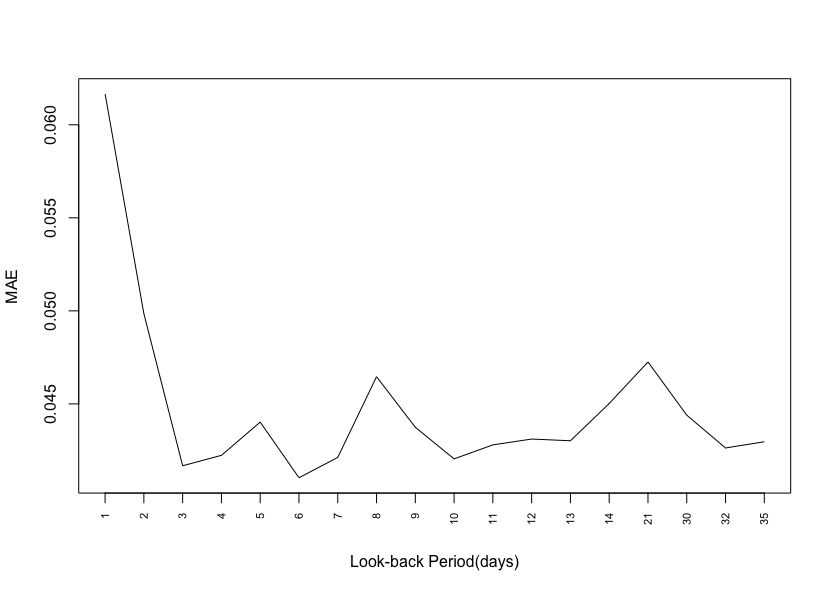
\includegraphics[width=\textwidth]{Figures/06Design/maeVlookback_chiwoza_med_light_20231128.png}
    \caption[MAE vs lookback-period Medical Light Chiwoza 20231128]{MAE vs Look-back period for medical light demand at Chiwoza 2023-11-28.}
    \label{fig:maeVlookback_chiwoza_med_light_20231128}
\end{figure}

\begin{figure}[]
    \centering
    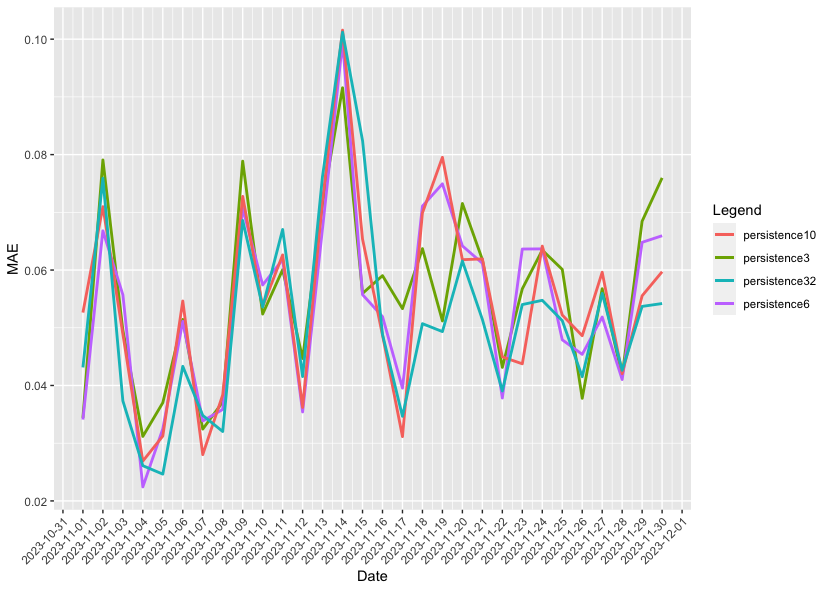
\includegraphics[width=\textwidth]{Figures/06Design/maeVlookback_chiwoza_med_light_202311.png}
    \caption[MAE vs look-back Medical light 202311]{MAE vs Look-back period for medical light demand at Chiwoza during the whole of November 2023. Using four persistence models with different look-back periods \textit{k}. (green:\textit{k}=3, purple:\textit{k}=6, red:\textit{k}=10), turquoise:\textit{k}=32)}
    \label{fig:maeVlookback_chiwoza_med_light202311}
\end{figure}

\begin{table}[]
    \centering
    \begin{tabular}{c|c}
         Look-back period (days)& Average MAE (W) \\
         3& 56\\
         6& 54\\
         10& 55\\
         32& 52
    \end{tabular}
    \caption[Average MAE persistence models]{Caption}
    \label{tab:avg_mae_chiwoza_med_persistence_2023}
\end{table}

\subsection{ARIMA Model}
The second model used for load forecasting is the ARIMA-model. The model was selected because it is purely statistical without the need for a priori data. As mentioned in \ref{seq:stat_forecasting}, an ARIMA model is a statistical forecasting model combining an auto-regressive and moving average model with a differentiating term. Through the analysis both intra- and inter-day periodicity was discovered for several of the meters, hence a SARIMA model is appropriate. To design a SARIMA model for each meter to be forecasted, the following terms must be determined
\begin{itemize}
    \item \textit{p}    -   The order of the auto-regressive model.
    \item \textit{d}    -   The differentiating order.
    \item \textit{q}    -   The order of the moving average model.
    \item \textit{P}    -   The order of the auto-regressive model shifted back one period.
    \item \textit{D}    -   The amount of terms one period back shifted to include directly.
    \item \textit{Q}    -   The order of the moving average model shifted back one period.
    \item \textit{s}    -   The period of the time-series.
\end{itemize}

Of these, only the time-series period, \textit{s}, is known in advance. From the analysis, it is known that the demand follows a daily cycle. The period is therefore equal to the number of samples within a day, which if done on an hourly basis equals 24.\\

The other parameters are to be obtained through a statistical analysis of the time-series for each meter. The first step of this process is to examine the original time-series for a given meter. Figure \ref{fig:con_ts_chiwoza_med_light_20231110-25} showcasing the consumption of medical lights at Chiwoza is a seemingly stationary time-series. The series oscillates, but there is no evident trend. This suggests stationarity. Further evidence can be found by using the augmented dicker-fuller test, where the results are shown in \ref{tab:result_dicker-fuller} strongly reject the null hypothesis of non-stationarity between the days. Figure \ref{fig:con_acf_h_chiwoza_med_light_20231110-25} confirms this, as the ACF decreases to zero after a few lags. This means that the auto-regressive and moving average model can be utilized without differentiating the time-series first. Although it is still possible that one can achieve better results by a differentiated time-series.\\


\begin{figure}[]
    \centering
    \includegraphics[width=\linewidth]{Figures/06Design/con_ts_chiwoza_med_light_20231110-25.png}
    \caption[Medical Light consumption Chiwoza 20231110-1125]{Consumption medical light Chiwoza as a time-series between 2023-11-10 and 2023-11-25.}
    \label{fig:con_ts_chiwoza_med_light_20231110-25}
\end{figure}

\begin{figure}[]
    \centering
    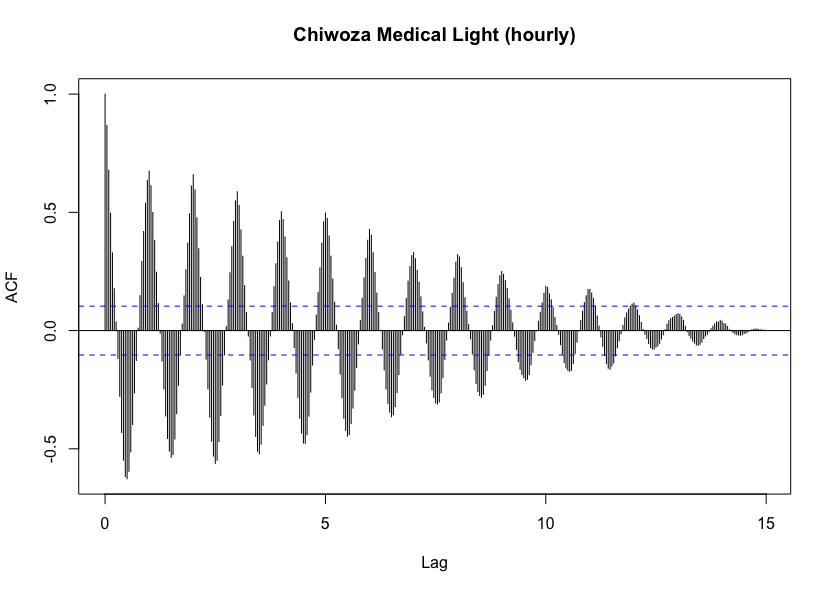
\includegraphics[width=\textwidth]{Figures/06Design/con_acf_h_chiwoza_med_light_20231110-25.png}
    \caption[ACF Medical Light consumption Chiwoza 20231110-1125]{ACF of the hourly consumption of the medical lights at Chiwoza between 2023-11-10 and 2023-11-25.}
    \label{fig:con_acf_h_chiwoza_med_light_20231110-25}
\end{figure}


\begin{table}[]
    \centering
    \begin{tabular}{c|c|c|c}
    Meter & DF & p-value & time range \\
    \hline
    Medical Lights Chiwoza & -9.0046 & <0.01 & 2023-11-10 - 2023-11-25
    \end{tabular}
    \caption[Dicker-Fuller test]{The results of the Augmented-Dicker-Fuller test}
    \label{tab:result_dicker-fuller}
\end{table}

Within a day, we know that there is a seasonal pattern. Looking at figure \ref{fig:con_acf_h_chiwoza_med_light_20231125} this means that the ACF does not decay, and an MA-model cannot be utilized. The PACF however, shown in figure \ref{fig:con_pacf_h_chiwoza_med_light_20231125} shows clear contributions from certain terms. A pure auto-regressive model combined with some seasonal terms is therefore a candidate. Differentiating the time-series and finding the ACF and PACF within a day produces the plots shown in figure \ref{fig:con_d_acf_pacf_h_chiwoza_med_light_20231125}. Here the ACF plot decays faster, meaning that a candidate with a differential term can be included.\\

\begin{figure}[]
  \centering

  % First Subfigure
  \begin{subfigure}{\textwidth}
    \centering
    \includegraphics[width=\linewidth]{Figures/06Design/con_acf_h_chiwoza_med_light_20231125.png}
    \caption[ACF Medical light consumption 20231110]{ACF of hourly medical light consumption Chiwoza at 2023-11-10.}
    \label{fig:con_acf_h_chiwoza_med_light_20231125}
  \end{subfigure}

  % Add some vertical space between the subfigures
  \vspace{0.5cm}

  % Second Subfigure
  \begin{subfigure}{\textwidth}
    \centering
    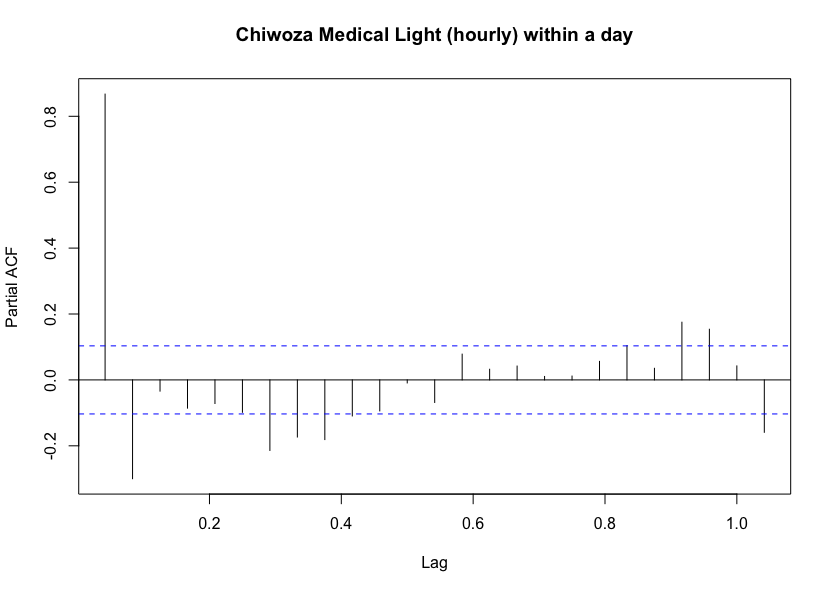
\includegraphics[width=\linewidth]{Figures/06Design/con_pacf_h_chiwoza_med_light_20231125.png}
    \caption[ACF Medical light consumption 20231110]{PACF of hourly medical light consumption Chiwoza at 2023-11-10.}
    \label{fig:con_pacf_h_chiwoza_med_light_20231125}
  \end{subfigure}

  \caption[ACF and PACF Medical light consumption 20231110]{ACF and PACF of hourly medical light consumption Chiwoza at 2023-11-10.}
  \label{fig:con_acf_pacf_h_chiwoza_med_light_20231125}
\end{figure}

\begin{figure}[]
  \centering

  % First Subfigure
  \begin{subfigure}{\textwidth}
    \centering
    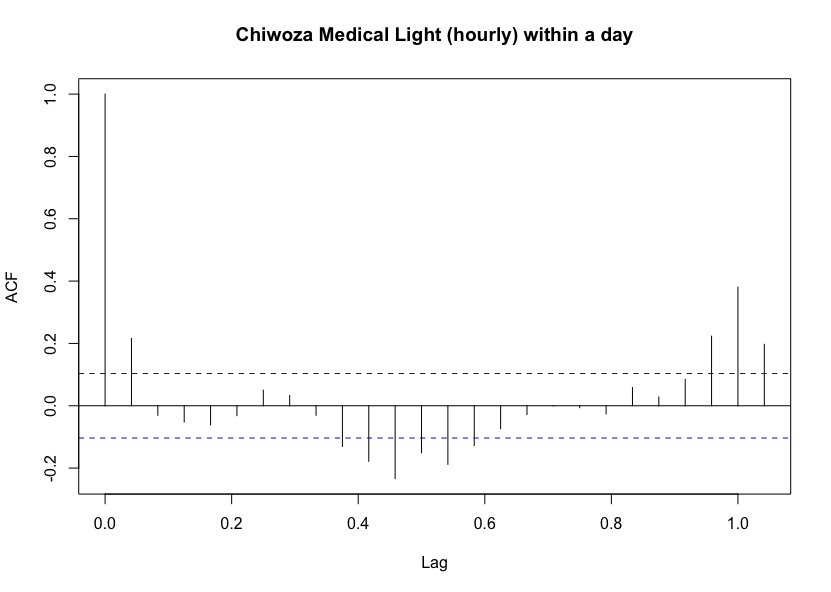
\includegraphics[width=\linewidth]{Figures/06Design/con_d_acf_h_chiwoza_med_light_20231125.png}
    \caption[ACF differentiated Medical light consumption 20231110]{ACF of differentiated hourly medical light consumption Chiwoza at 2023-11-10.}
    \label{fig:con_d_acf_h_chiwoza_med_light_20231125}
  \end{subfigure}

  % Add some vertical space between the subfigures
  \vspace{0.5cm}

  % Second Subfigure
  \begin{subfigure}{\textwidth}
    \centering
    \includegraphics[width=\linewidth]{Figures/06Design/con_d_pacf_h_chiwoza_med_light_20231125.png}
    \caption[PACF differentiated medical light consumption 20231110]{PACF of differentiated  hourly medical light consumption Chiwoza at 2023-11-10.}
    \label{fig:con_d_pacf_h_chiwoza_med_light_20231125}
  \end{subfigure}

  \caption[ACF and PACF differentiated medical light consumption 20231110]{ACF and PACF of differentiated hourly medical light consumption Chiwoza at 2023-11-10.}
  \label{fig:con_d_acf_pacf_h_chiwoza_med_light_20231125}
\end{figure}

Section \ref{seq:tuning_arima} outlines the process of finding the \textit{p} and \textit{q} values of the model using the partial auto-correlation function (PACF) and the auto-correlation function(ACF) respectively. From figure \ref{fig:con_d_acf_pacf_h_chiwoza_med_light_20231125} we see that ARIMA(1,1,2)(1,1,1) can be a candidate. There is however still seasonality apparent in figure \ref{fig:con_d_acf_h_chiwoza_med_light_20231125}. Differentiating the time-series again removes all intra-day seasonality, as seen in figure \ref{fig:con_d2_acf_h_chiwoza_med_light_20231125} by the complete decay of the ACF besides the full lag. Combined with the PACF plot in figure \ref{fig:con_d2_pacf_h_chiwoza_med_light_20231125} we see that ARIMA(1,2,2)(1,1,1) could be another candidate. \\

\begin{figure}][]
  \centering

  % First Subfigure
  \begin{subfigure}{\textwidth}
    \centering
    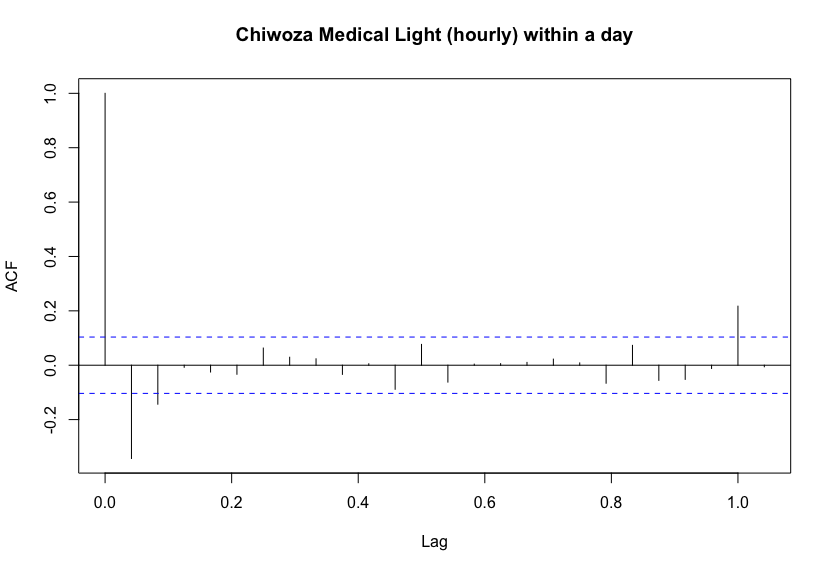
\includegraphics[width=\linewidth]{Figures/06Design/con_d2_acf_h_chiwoza_med_light_20231125.png}
    \caption[ACF second order differentiated medical consumption 20231110]{ACF of second order differentiated hourly medical light consumption Chiwoza at 2023-11-10.}
    \label{fig:con_d2_acf_h_chiwoza_med_light_20231125}
  \end{subfigure}

  % Add some vertical space between the subfigures
  \vspace{0.5cm}

  % Second Subfigure
  \begin{subfigure}{\textwidth}
    \centering
    \includegraphics[width=\linewidth]{Figures/06Design/con_d2_pacf_h_chiwoza_med_light_20231125.png}
    \caption[PACF second order differentiated medical consumption 20231110]{PACF of second order differentiated  hourly medical light consumption Chiwoza at 2023-11-10.}
    \label{fig:con_d2_pacf_h_chiwoza_med_light_20231125}
  \end{subfigure}

  \caption[ACF and PACF second order differentiated medical consumption 20231110]{ACF and PACF of second order differentiated hourly medical light consumption Chiwoza at 2023-11-10.}
  \label{fig:con_d2_acf_pacf_h_chiwoza_med_light_20231125}
\end{figure}

The three candidates listed in table \ref{tab:arima_candidate_chiwoza_med_light} can be implemented and tested over a wider time period. Model III looks clearly worse from the plot, but it is difficult separating I and II. From table \ref{tab:arima_candidate_mae_chiwoza_med_light} we see that model II performed slightly better on average MAE over the month of November. It also has a lower maximum MAE than model I. Of the ARIMA models, only I and II managed to beat the baseline set by the persistence model. Looking at the forecasted time-series for November from model II versus the actual time-series in figure \ref{fig:atVSft_chiwoza_medical_light_202311} , the model has acceptable performance. 

\begin{table}[]
    \centering
    \begin{tabular}{c|c}
         \#& model \\
         \hline
         I& ARIMA(2,0,0)(1,1,1)\\
         II& ARIMA(1,1,2)(1,1,1)\\
         III& ARIMA(1,2,2)(1,1,1)\\
    \end{tabular}
    \caption[ARIMA candidates medical light demand Chiwoza]{ARIMA model candidates for medical light demand Chiwoza}
    \label{tab:arima_candidate_chiwoza_med_light}
\end{table}

\begin{figure}[]
    \centering
    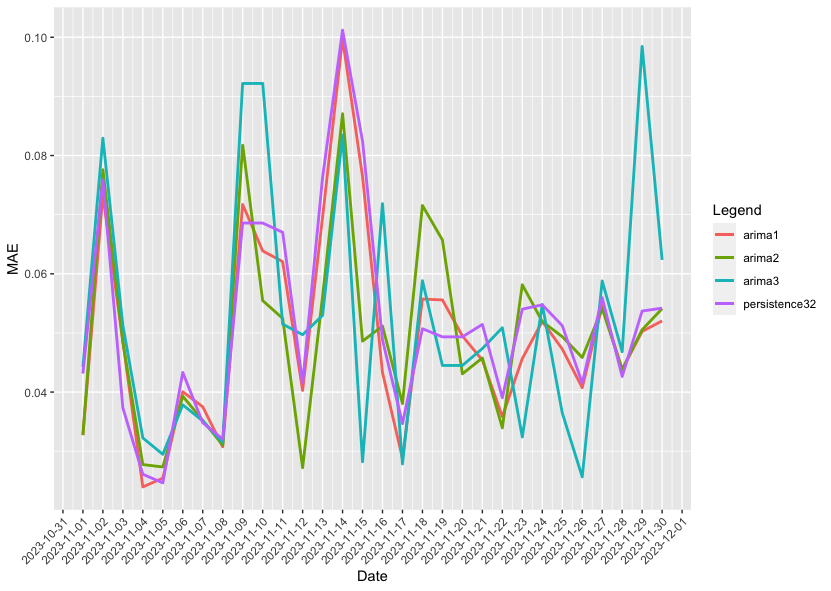
\includegraphics[width=\textwidth]{Figures/06Design/mae_arima_chiwoza_med_light_202311.png}
    \caption[MAE ARIMA candidates medical light demand Chiwoza]{MAE of the 3 ARIMA models listed in \ref{tab:arima_candidate_chiwoza_med_light} over the month of November 2023.Included is also the MAE of a persistence model with look-back period of 32 days}
    \label{fig:mae_arima_chiwoza_med_light_202311}
\end{figure}

\begin{table}[]
    \centering
    \begin{tabular}{c|c}
         \#& average MAE (W) \\
         \hline
         I& 49\\
         II& 49\\
         III& 52\\
         $persistence_{32}$& 52\\
    \end{tabular}
    \caption[Average MAE ARIMA candidates and persistence model medical light demand Chiwoza]{ARIMA model candidates' MAE for medical light demand estimation over the month of November at Chiwoza. Included is the average MAE of a persistence model with look-back period of 32 days.}
    \label{tab:arima_candidate_mae_chiwoza_med_light}
\end{table}

\begin{figure}[]
    \centering
    \includegraphics[width=\textwidth]{Figures/06Design/atVSft_chiwoza_medical_light_202311.png}
    \caption[Actual vs Forecasted medical light demand]{The actual hourly consumption vs the forecasted demand from the ARIMA model II in \ref{tab:arima_candidate_chiwoza_med_light} for medical light consumption Chiwoza November 2023.}
    \label{fig:atVSft_chiwoza_medical_light_202311}
\end{figure}

As mentioned earlier in this section, this process of selecting ARIMA candidates, comparing them against each other and a persistence model has to be repeated for all the loads connected to a system that is to be forecasted. The result of this is shown in \ref{tab:load_forecasting_results_chiwoza}. In section \ref{seq:periodicity}, some loads, like the Guardian shelter Socket were found to have a strong weekday pattern. To accommodate for this, the ARIMA was modified to include this behavior. The algorithm, shown in \ref{alg:arima_forecast_periodic}, runs a different ARIMA model for weekdays and weekends. Furthermore, when gathering historic data for its forecast, it discards days it has been asked to ignore. In \ref{fig:forecasting_results_chiwoza_guard_socket} this is seen as a model which is able to handle the shape of high consumption during the week and none during the weekend.

\begin{algorithm}
\caption{ARIMA forecaster weekday periodic (Pseudocode)}\label{alg:arima_forecast_periodic}
\begin{algorithmic}
    \State$dow = dayOfWeek(date) $
    \If{$dow == Sat | dow == Sun$}
        \State$ignoreDays = (Mon,Tue,Wed,Thu,Fri)$
        \State$model \gets arimaWeekendParam$
    \Else
        \State$ignoreDays = (Sat,Sun)$
        \State$model \gets arimaWeekdayParam$
    \EndIf
    \State$historicData \gets getHistoricData(ignoreDays)$
    \State$forecast \gets arimaForecast(model, historicData)$
\end{algorithmic}
\end{algorithm}

\begin{figure}
% First Subfigure
    \begin{subfigure}{\textwidth}
    \centering
    \includegraphics[width=\linewidth]{Figures/06Design/con_ts_chiwoza_staff_light1_20231101-26.png}
    \caption{Light consumption at staff house 1 Chiwoza during November.}
    \label{fig:con_ts_chiwoza_staff_light1_20231101-26}
  \end{subfigure}

  % Add some vertical space between the subfigures
  \vspace{0.5cm}

  % Second Subfigure
  \begin{subfigure}{\textwidth}
    \centering
    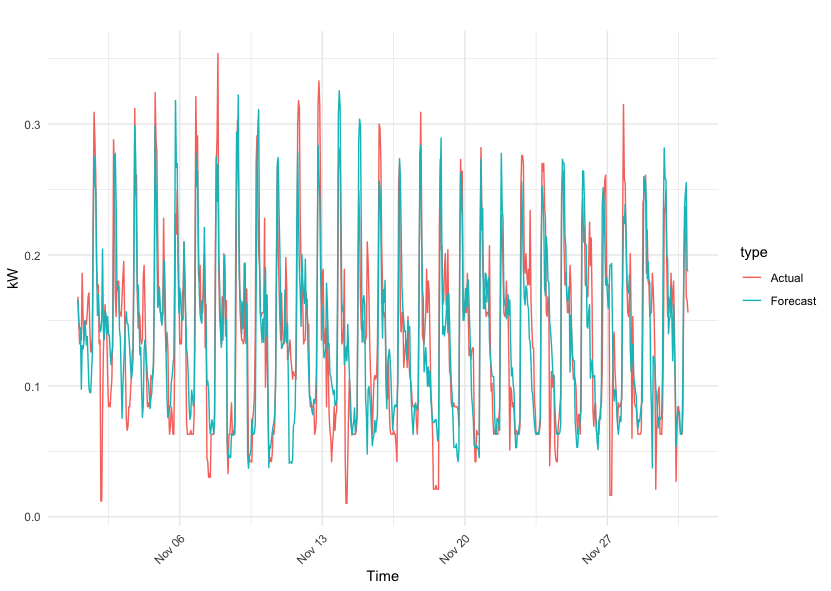
\includegraphics[width=\linewidth]{Figures/06Design/atVSft_chiwoza_staff_light1_202311.png}
    \caption{The actual vs the forecasted hourly light consumption for Chiwoza Staff house 1.}
    \label{fig:atVSft_chiwoza_staff_light1_202311}
  \end{subfigure}

  \caption[Light consumption staff house 1 forecasting]{Starting point and result load forecasting for light consumption for Chiwoza Staff house 1.}
  \label{fig:forecasting_results_chiwoza_staff_light1}
\end{figure}

\begin{figure}
% First Subfigure
    \begin{subfigure}{\textwidth}
    \centering
    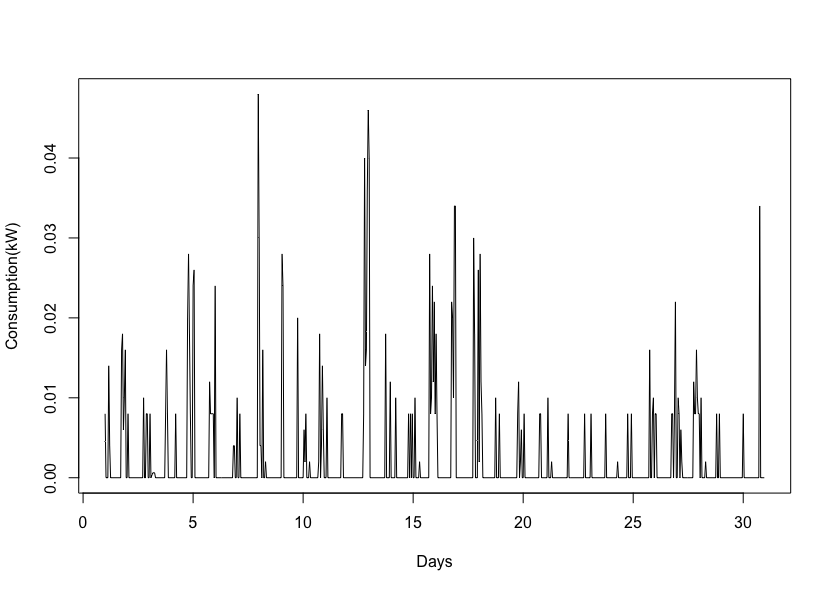
\includegraphics[width=\linewidth]{Figures/06Design/con_ts_chiwoza_staff_light2_20231101-30.png}
    \caption{Light consumption at staff house 2 Chiwoza during November.}
    \label{fig:con_ts_chiwoza_staff_light2_202311}
  \end{subfigure}

  % Add some vertical space between the subfigures
  \vspace{0.5cm}

  % Second Subfigure
  \begin{subfigure}{\textwidth}
    \centering
    \includegraphics[width=\linewidth]{Figures/06Design/atVSft_chiwoza_staff_light2_202311.png}
    \caption{The actual vs the forecasted hourly light consumption for Chiwoza Staff house 2.}
    \label{fig:atVSft_chiwoza_staff_light2_202311}
  \end{subfigure}

  \caption[Light consumption staff house 2 forecasting]{Starting point and result load forecasting for light consumption for Chiwoza Staff house 2.}
  \label{fig:forecasting_results_chiwoza_staff_light2}
\end{figure}

\begin{figure}
% First Subfigure
    \begin{subfigure}{\textwidth}
    \centering
    \includegraphics[width=\linewidth]{Figures/06Design/con_ts_chiwoza_staff_light3_202311.png}
    \caption{Light consumption at staff house 3 Chiwoza during November.}
    \label{fig:con_ts_chiwoza_staff_light3_20231001-20}
  \end{subfigure}
  
  % Add some vertical space between the subfigures
  \vspace{0.5cm}

  % Second Subfigure
  
  \begin{subfigure}{\textwidth}
    \centering
    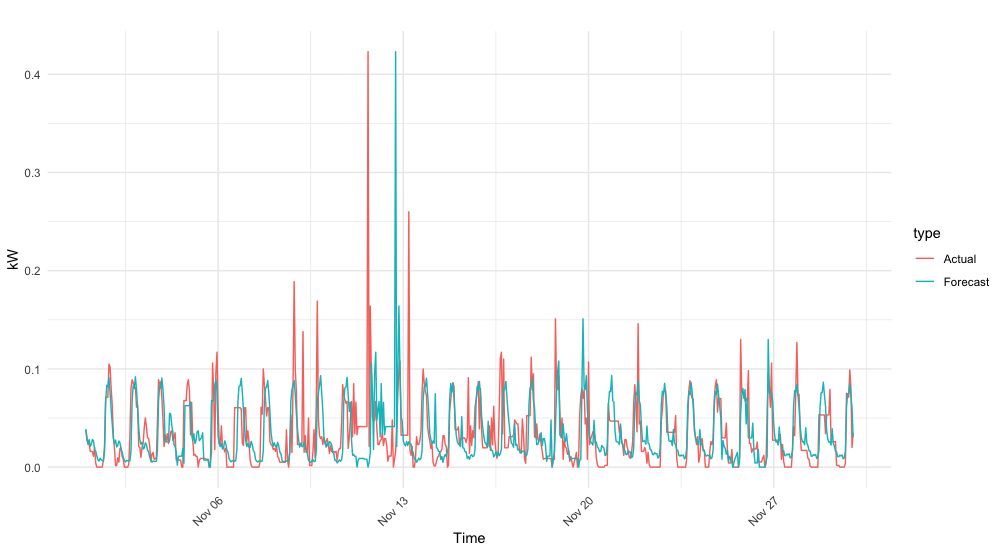
\includegraphics[width=\linewidth]{Figures/06Design/atVSft_chiwoza_staff_light3_202311.png}
    \caption{The actual vs the forecasted hourly light consumption for Chiwoza Staff house 3.}
    \label{fig:atVSft_chiwoza_staff_light3_20231001-20}
  \end{subfigure}


  \caption[Light consumption staff house 3 forecasting]{Starting point and result load forecasting for light consumption for Chiwoza Staff house 3.}
  \label{fig:forecasting_results_chiwoza_staff_light3}
\end{figure}

\begin{figure}
% First Subfigure
    \begin{subfigure}{\textwidth}
    \centering
    \includegraphics[width=\linewidth]{Figures/06Design/con_ts_chiwoza_fence_light_202310.png}
    \caption{Hourly consumption for the Chiwoza Fence light during October 2023.}
    \label{fig:con_ts_chiwoza_fence_light_202310}
  \end{subfigure}

  % Add some vertical space between the subfigures
  \vspace{0.5cm}

  % Second Subfigure
  \begin{subfigure}{\textwidth}
    \centering
    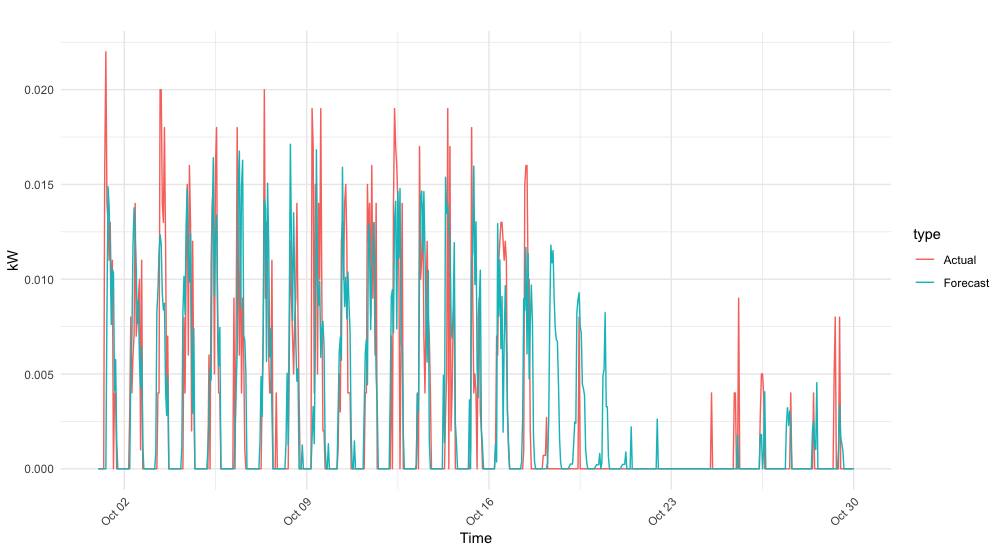
\includegraphics[width=\linewidth]{Figures/06Design/atVSft_chiwoza_fence_light_202310.png}
    \caption{The actual vs the forecasted hourly consumption for the Chiwoza Fence light.}
    \label{fig:atVSft_chiwoza_fence_light_202310}
  \end{subfigure}

  \caption[Fence Light consumption forecasting]{Starting point and result load forecasting for hourly consumption for the Chiwoza Fence light.}
  \label{fig:forecasting_results_chiwoza_fence_light}
\end{figure}

\begin{figure}
% First Subfigure
    \begin{subfigure}{\textwidth}
    \centering
    \includegraphics[width=\linewidth]{Figures/06Design/con_ts_chiwoza_guard_light_202311.png}
    \caption{Hourly consumption for the Chiwoza Guardian Shelter light during November 2023.}
    \label{fig:con_ts_chiwoza_guard_light_202311}
  \end{subfigure}

  % Add some vertical space between the subfigures
  \vspace{0.5cm}

  % Second Subfigure
  \begin{subfigure}{\textwidth}
    \centering
    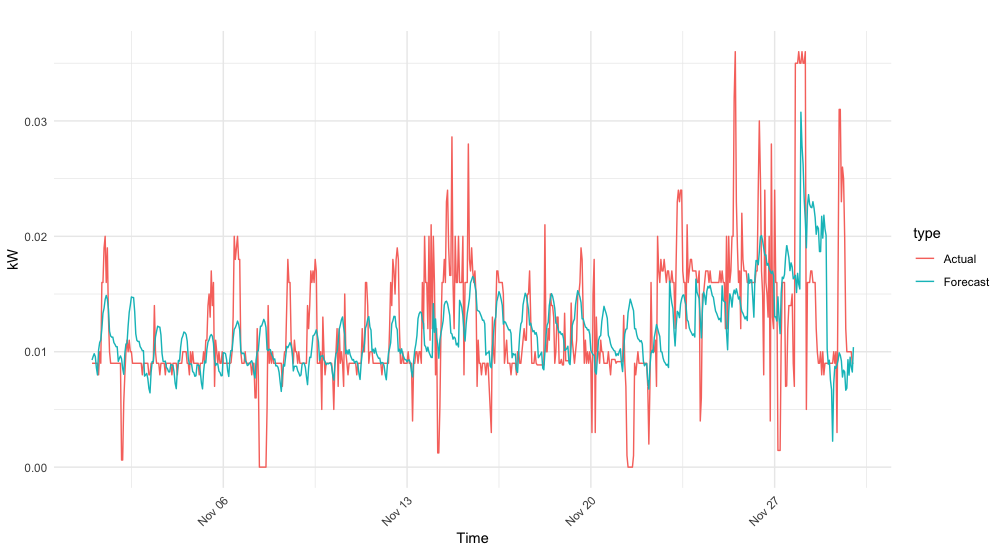
\includegraphics[width=\linewidth]{Figures/06Design/atVSft_chiwoza_guard_light_202311.png}
    \caption{The actual vs the forecasted hourly consumption for the Chiwoza Guardian Shelter light.}
    \label{fig:atVSft_chiwoza_guard_light_202311}
  \end{subfigure}

  \caption[Guardian Shelter consumption forecasting]{Starting point and result load forecasting for hourly consumption for the Chiwoza Guardian Shelter light.}
  \label{fig:forecasting_results_chiwoza_guard_light}
\end{figure}

\begin{figure}
% First Subfigure
    \begin{subfigure}{\textwidth}
    \centering
    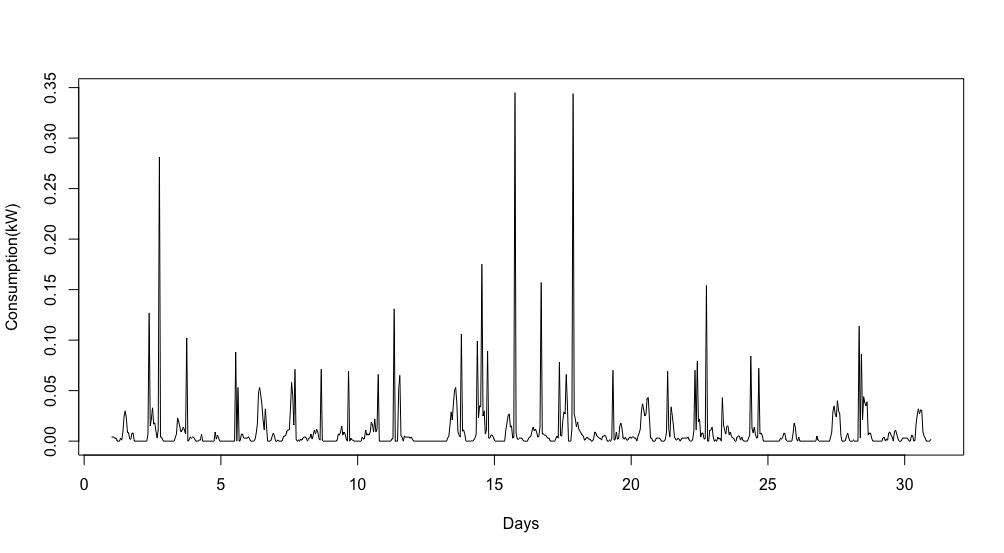
\includegraphics[width=\linewidth]{Figures/06Design/con_ts_chiwoza_med_socket_202311.png}
    \caption{Hourly consumption for the Chiwoza medical socket during November 2023.}
    \label{fig:con_ts_chiwoza_med_socket_202311}
  \end{subfigure}

  % Add some vertical space between the subfigures
  \vspace{0.5cm}

  % Second Subfigure
  \begin{subfigure}{\textwidth}
    \centering
    \includegraphics[width=\linewidth]{Figures/06Design/atVSft_chiwoza_med_socket_202311.png}
    \caption{The actual vs the forecasted hourly consumption for the Chiwoza medical socket.}
    \label{fig:atVSft_chiwoza_med_socket_202311}
  \end{subfigure}

  \caption[Medical light socket forecasting]{Starting point and result load forecasting for hourly consumption for the Chiwoza Medical socket.}
  \label{fig:forecasting_results_chiwoza_medical_socket}
\end{figure}

\begin{figure}
% First Subfigure
    \begin{minipage}{0.9\textwidth} % Adjust the width as needed
    \begin{subfigure}{\textwidth}
        \centering
        \includegraphics[width=\linewidth]{Figures/06Design/con_ts_chiwoza_staff_socket3_202311.png}
        \caption{Hourly consumption for the Chiwoza staff socket 3 during November 2023.}
        \label{fig:con_ts_chiwoza_staff_socket3_202311}
    \end{subfigure}
    \end{minipage}

  % Add some vertical space between the subfigures
  \vspace{0.5cm}

  % Second Subfigure
    \begin{minipage}{0.9\textwidth} % Adjust the width as needed
    \begin{subfigure}{\textwidth}
        \centering
        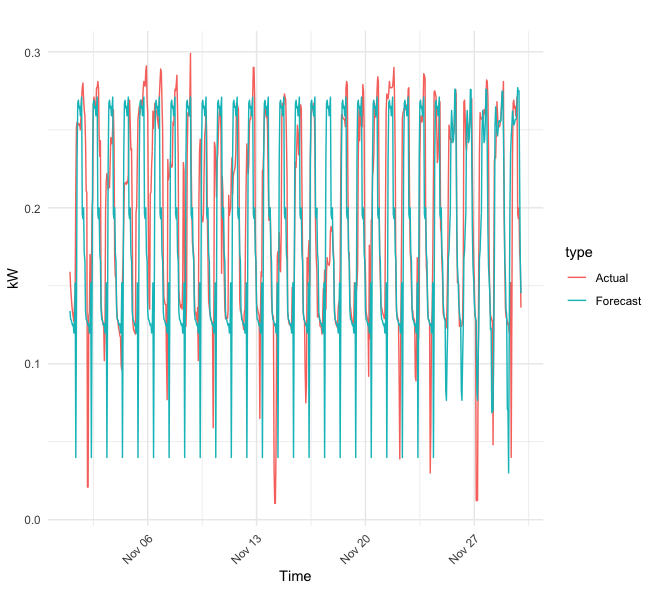
\includegraphics[width=\linewidth]{Figures/06Design/atVSft_chiwoza_staff_socket3_202311.png}
        \caption{The actual vs the forecasted hourly consumption for the Chiwoza staff socket 3.}
        \label{fig:atVSft_chiwoza_staff_socket3_202311}
    \end{subfigure}
    \end{minipage}


  \caption[Staff socket 3 consumption forecasting]{Starting point and result load forecasting for hourly consumption for the Chiwoza staff socket 3.}
  \label{fig:forecasting_results_chiwoza_staff_socket3}
\end{figure}

\begin{figure}
% First Subfigure
    \begin{subfigure}{\textwidth}
    \centering
    \includegraphics[width=\linewidth]{Figures/06Design/con_ts_chiwoza_guard_socket_20231119-1216.png}
    \caption{Hourly consumption for the Chiwoza guardian shelter socket 3 from November 19th to December 16th 2023.}
    \label{fig:con_ts_chiwoza_guard_socket_20231119-1216}
  \end{subfigure}

  % Add some vertical space between the subfigures
  \vspace{0.5cm}

  % Second Subfigure
  \begin{subfigure}{\textwidth}
    \centering
    \includegraphics[width=\linewidth]{Figures/06Design/atVSft_chiwoza_guard_socket_20231119-1216.png}
    \caption{The actual vs the forecasted hourly consumption for the Chiwoza guardian shelter socket 3 from November 19th to December 16th 2023.}
    \label{fig:atVSft_chiwoza_guard_socket_20231119-1216}
  \end{subfigure}

  \caption[Guardian shelter socket consumption forecasting]{Starting point and result load forecasting for hourly consumption for the Chiwoza guardian shelter socket 3 from November 19th to December 16th 2023.}
  \label{fig:forecasting_results_chiwoza_guard_socket}
\end{figure}

\begin{table}[]
    \centering
    \begin{tabular}{c|c|c|c|c}
        Load & Forecasting model & Average MAE (W) & Average (W) & Plot  \\
        \hline
        Medical Light   & ARIMA(1,1,2)(1,1,1) & 49  &  113  &   \ref{fig:atVSft_chiwoza_medical_light_202311}\\
        Medical Socket  & ARIMA(2,1,1)(0,1,1) & 10  &   11  &   \ref{fig:forecasting_results_chiwoza_medical_socket}\\
        Staff Light 1   & ARIMA(1,0,0)(1,1,2) & 26  &  46   &   \ref{fig:forecasting_results_chiwoza_staff_light1}\\
        Staff Light 2   & ARIMA(1,0,0)(1,1,1) & 3   &  6    &   \ref{fig:forecasting_results_chiwoza_staff_light2}\\
        Staff Light 3   & ARIMA(1,0,0)(1,1,0) & 18  &  33   &   \ref{fig:forecasting_results_chiwoza_staff_light3}\\
        Staff Socket 3  & ARIMA(2,0,0)(2,1,0) & 28  &  199  &   \ref{fig:forecasting_results_chiwoza_staff_socket3}\\
        Fence Light     & ARIMA(1,0,1)(2,1,0) & 1.7 &  2.4  &   \ref{fig:forecasting_results_chiwoza_fence_light}\\
        Guardian Shelter Light  & ARIMA(6,1,1)(0,1,1) & 3   &   12  &   \ref{fig:forecasting_results_chiwoza_guard_light}\\
        Guardian Shelter Socket  & ARIMA(1,0,1)(0,1,2) & 1.4  &  1.8  &   \ref{fig:forecasting_results_chiwoza_guard_socket}\\
    \end{tabular}
    \caption[Chiwoza demand forecasting results]{Loads at Chiwoza with their deduced forecast model.}
    \label{tab:load_forecasting_results_chiwoza}
\end{table}



The forecasting yields large errors, especially when forecasting loads with large spikes in consumption, such as the Chiwoza medical socket seen in figure \ref{fig:forecasting_results_chiwoza_medical_socket}. Here the forecast has the correct shape, but misses the timing. Sudden and high spikes in consumption are expected to be hard to forecast from statistical data alone. 

\subsection{Forecast update}
In the results from the previous section, demand has been forecasted once every day, and compared to the actual. Instead in the proposed control system, a new forecast will be made every time there is a new measurement. This is done by including the measurement in the historic data used to make the forecast. This frequency of updated forecasts will increase accuracy. In figure \ref{fig:atVSft_chiwoza_med_light20231125} the forecast for medical light demand at Chiwoza on the 25th of November 2023 is updated each hour. In this forecast, the MAE is reduced by about 84\%, from 49 to 7.8, compared to the average MAE for the daily forecasts between October 23rd- December 23rd 2023.\\
 

\begin{figure}
    \centering
    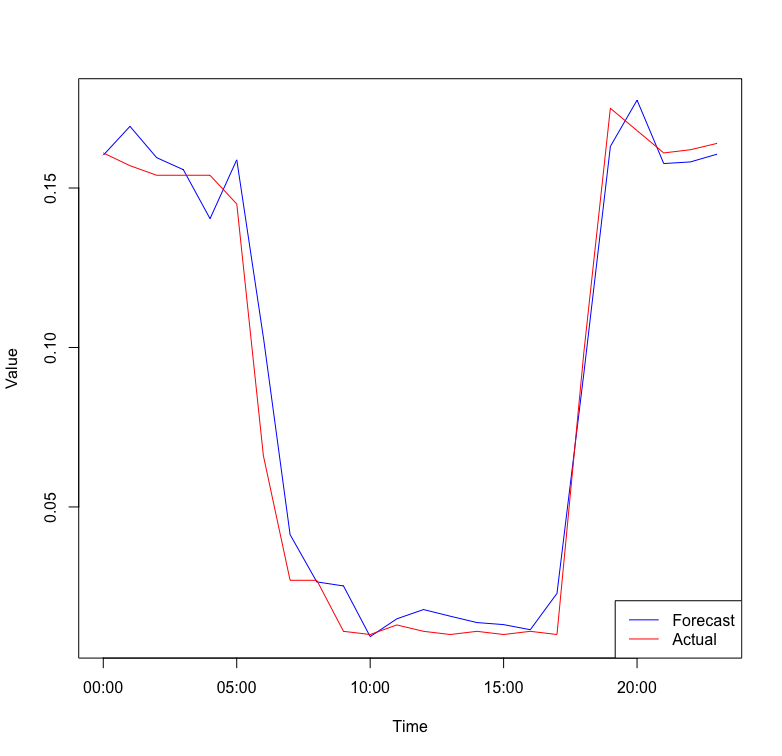
\includegraphics[width=\linewidth]{Figures/06Design/atVSft_chiwoza_med_light20231125.png}
    \caption[Hourly updated forecast Chiwoza medical light]{Hourly updated forecast for medical light demand at Chiwoza for November 25th 2023. $MAE=7.8W$}
    \label{fig:atVSft_chiwoza_med_light20231125}
\end{figure}



\section{Production analysis}\label{seq:prod_analysis}

The sole production module in the systems is the PV-modules. An outline of its dynamics and connection to irradiance is given in section \ref{seq:pv_and_irradiance}. As mentioned in that section, irradiance can be classified into different types. Each of these has its effect on PV production and is measured individually with the right measurement devices.\\

There are no measurement devices for irradiance at the sites, but there exists \textit{geographic information systems} (GIS)-tools such as the European PVGIS\cite{pvgis} that give average daily values each month based upon large weather databases. Figure \ref{fig:irradiance_daily_pvgis_chiwoza_dec} displays the downloaded average daily irradiance downloaded from PVGIS at the Chiwoza during December.\\

The daily average irradiance will have a seasonal trend, given the changing position between the Sun and the Earth. Figure \ref{fig:irradiance_monthly_pvgis_chiwoza_2020} shows how the irradiance varies throughout the year. It is therefore important to gather the daily average corresponding to the correct month.

\begin{figure}
    \centering
    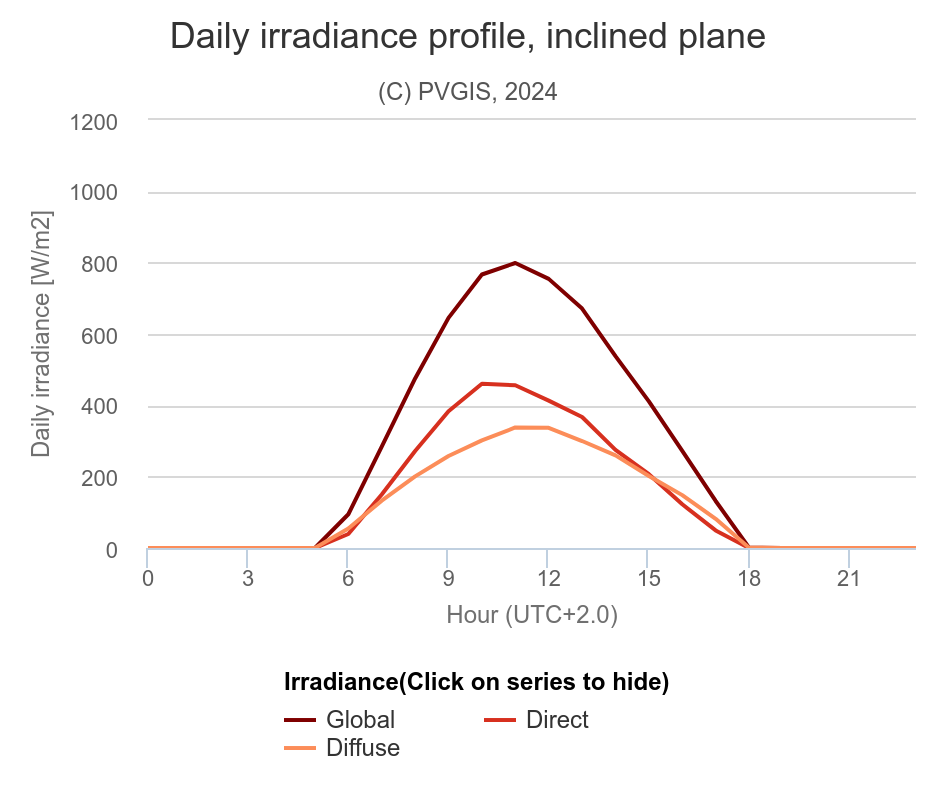
\includegraphics[width=\linewidth]{Figures/06Design/irradiance_daily_pvgis_chiwoza_dec.png}
    \caption[Daily irradiance Chiwoza]{Average daily irradiance Chiwoza for December. Figure downloaded from PVGIS\cite{pvgis}}
    \label{fig:irradiance_daily_pvgis_chiwoza_dec}
\end{figure}

\begin{figure}
    \centering
    \includegraphics[width=\linewidth]{Figures/06Design/irradiance_monthly_pvgis_chiwoza_2020.png}
    \caption[Monthly irradiance Chiwoza 2020]{Total monthly irradiance Chiwoza 2020. Figure downloaded from PVGIS\cite{pvgis}}
    \label{fig:irradiance_monthly_pvgis_chiwoza_2020}
\end{figure}

There is a strong connection between weather and PV production, seen from for instance equation \ref{eq:irradiance}. However, there are no weather measurement devices at the sites due to the cost of such equipment. Information about the weather is gained through the online databases of the Norwegian Meteorological Agency. Both weather forecasts and weather measurements are fetched. Both of these have an inherent quite large uncertainty.\\

Besides the lack of measurements, another complicating factor for production analysis is the underutilization at the sites. The sites cannot deliver more power than consumed by the loads, stored in the battery or lost in the system. Hence, as load consumption, in general, is low, the production is far below its full potential. This can be seen in figure \ref{fig:yieldVSirradiance_day_chiwoza_202309}. The figure shows the average, maximum and minimum recorded production for each hour of the day in September 2023. This is plotted against the GHI fetched from PVGIS\cite{pvgis}. While the scale between irradiance and production is different, the important thing is the shape of the irradiance curve versus the production curves. While the points of the GHI show a quadratic curve, the production peaks early in the day, and then tapers off quickly. This is because the system uses a lot of power early in the day, to charge the battery, but once the battery is charged up to 90\% the production drops sharply, only supplying the low amount of load connected during the day. The peak toward the end of the day is because of the charging algorithm of the batteries outlined in section \ref{seq:current_syst}. If the load was not a limiting factor, so that all available power was utilized, one would expect a production curve with a similar curve to the irradiance curve due to their tight relationship.

\begin{figure}
  \centering
    \includegraphics[width=\linewidth]{Figures/06Design/yieldVSirradiance_day_chiwoza_202309.png}
    \caption[Yield vs irradiance September 2023]{Average, max and min yield vs GHI Chiwoza September 2023}
    \label{fig:yieldVSirradiance_day_chiwoza_202309}
\end{figure}

\section{Forecasting production}\label{seq:prod_forecasting}
The systems are dependent on the PV-production to satisfy load demand.  Knowing the timing and magnitude of the production is critical to make informed decisions on the operation of the systems. As mentioned in the analysis, the production is limited by the load consumption. As the goal of the thesis is to find how load can be moved, added and controlled, the current production is therefore far less interesting than the potential production.\\



Similarly as for the load forecasting, one would expect an auto-regressive feature to the production. This would suggest that a statistical forecasting algorithm, such as the ARIMA used for load forecasting, could be appropriate. However, given the discussion on underutilization from the previous section, measured production is poorly suited to estimate the maximum potential production. Assuming unlimited production during the early morning hours, when the battery is charging, one could find the relationship between the production during those hours, and the irradiance curve, and use that ratio to predict future potential production. However, as this varies a lot with the weather conditions in the early morning hours and usage, this approach is prone to over-fitting and errors. Statistical forecasting of production is therefore sub-optimal as long as no non-load-limited production measurements are done at the sites.\\

Luckily, it is far easier to deduce a physical model of production than for load, given the unpredictable nature of load consumption. A physical model removes the need for past data for forecasting. 

The physical model is based on the approach in section \ref{seq:physical_forecasting}, with especially equation \ref{eq:pv_power_full} showing the relationship between irradiance and power. The irradiance is modified by equation \ref{eq:irradiance} to include the effect of the cloud cover. In total, the physical model for the PV-production from a PV-module with $n_{panels}$ PV-panels is defined in \ref{eq:pv_prod_physical_model}. The inputs to these models are the parameters relating to the panels, global- and diffuse irradiance and cloud cover. The panel parameters such as $P_{STC}$, $G_STC$ and $n_panels$ are known, while the $G_{GHI}$ and $G_{DHI}$ do not change from day to day within a month. The only factor modifying the model to give a variable daily estimate is the cloud cover. This is gathered from weather forecasts. 

\begin{equation}
    P_{PV} = \frac{P_{STC}}{G_{STC}}(G_{GHI}(1-f)+G_{DHI}f)n_{panels}
    \label{eq:pv_prod_physical_model}
\end{equation}

As mentioned in section \ref{seq:prod_analysis}, actual measured production at the site is a poor comparison to estimated potential production because it is limited by consumption. This makes it difficult to test the model. However, if one assumes the model is reasonable, the model would given accurate weather measurements give an accurate estimate of potential production. It is then possible to test the model with weather measurements against the model using weather forecasts. In figure \ref{fig:prod_atVSft_chiwoza_20231201} the model is tested with a weather forecast from the start of the period plotted against a weather measurement taken at each hour during the day. The weather measurement, gathered from satellite data\cite{met.no}, is the best available measurement of the weather for each hour. Hence, the model based on the measurement represents the best available estimate of the potential production given actual weather data and not limited by consumption. The figure shows that during the first few hours, the forecast is identical to the actual estimate. Later on, the difference between the two varies in both directions. The cumulative difference indicates that the forecast estimates a lower potential production for this day. 

\begin{figure}
    \centering
    \includegraphics[width=\textwidth]{Figures/06Design/prod_atVSft_chiwoza_20231201.png}
    \caption[Forecasted vs estimated potential production]{The production estimate based on actual weather measurement versus the forecasted production based on the weather forecast for Chiwoza December 1st 2023. Included is also the cumulative difference between the two. MAE = 626W}
    \label{fig:prod_atVSft_chiwoza_20231201}
\end{figure}


\subsection{Forecast update}
Similarly, as for load forecasting, the production forecast is updated every time there is a new weather or production measurement. This is shown for December 1st 2023 in figure \ref{fig:atVSft_prod_chiwoza20231220} where an hourly updated forecast leads to more halving of MAE compared to the forecast over the same period in figure \ref{fig:prod_atVSft_chiwoza_20231201}.

\begin{figure}
    \centering
    \includegraphics[width=\textwidth]{Figures/06Design/atVSft_prod_chiwoza20231220.png}
    \caption[Forecasted vs estimated potential production hourly update]{The production estimate based on actual weather measurement versus the forecasted production based on the weather forecast for Chiwoza December 1st 2023. The forecast is updated every hour. $MAE = 263W$}
    \label{fig:atVSft_prod_chiwoza20231220}
\end{figure}

\subsection{System Loss}
The model in \ref{eq:pv_prod_physical_model} neglects energy lost within the system. There are plenty of factors leading to a reduction in the energy available. While we know that the inverter has a peak efficiency of 96\% and the solar charger has a peak efficiency of 99\% from the datasheet, the wiring and panel losses are unknown. There is therefore not enough information available to accurately estimate the system losses in the current system. In \textit{(Chimtavee A. and Ketjoy, N,2012)}, the authors found an average loss of $26.27\%$ over a whole year.\cite{Chimtavee2012-gg} Modifying the production forecast in \ref{eq:pv_prod_physical_model} by a constant loss factor \textit{h}, yields model shown in equation \ref{eq:pv_prod_physical_model_loss}.

\begin{equation}
    P_{PV} = \frac{P_{STC}}{G_{STC}}(G_{GHI}(1-f)+G_{DHI}f)n_{panels}*(1-h)
    \label{eq:pv_prod_physical_model_loss}
\end{equation}

\section{Optimization}\label{sec:optimization}

As shown in \ref{fig:control_syst}, the optimizer is fed the load and production forecast from the forecasters. While the production and demand in the system are naturally continuous variables the forecasts are discrete vectors giving the value for every time-step within the prediction horizon.  The optimizer is tasked with finding the optimal plan for each time-step within the prediction horizon, based on the KPIs shown in \ref{tab:KPI}. There are several ways to design an optimizer algorithm, including rule-based approaches, machine-learning, continuous optimization and integer programming.\\

The current control system is rule-based. A natural design choice would be to modify the current control system to address some of the weaknesses described in section \ref{sec:weaknesses_current_syst}. The weaknesses however, especially the one about the inability to adapt to changing conditions would be difficult to address without including forecasting and load prioritization as part of the algorithm. Because this is a core functionality, doing so would amount to an almost complete re-design of the current control system. 

A rule-based control system divides the state space into distinct sections and attributes a set of actions to each section. This can be illustrated by a Finite State Machine as done for the current charge control shown in figure \ref{fig:current_battery_control_FSM}. An issue with rule-based control is that their complexity and rigidity increase quickly with the amount of possible distinct states and transitions between states.\cite{Casini2022-bs} Hence another approach outside the rule-based paradigm is proposed in this thesis.\\

While machine learning has been proposed by several papers for energy management systems, as in \textit{(Philipo GH. et al., 2022)},\cite{Philipo2022-rx} it was not chosen for this thesis because of the tuning of such a system can be oblique. Therefore, an optimisation approach was chosen, inspired by the works of \textit{(Salazar A. et al.,2020)} and \textit{(Sadek SM. et al., 2020)} found in the literature survey. Both continuous and discrete optimisation (Integer Programming) was attempted, however with the latter there was an issue of solution stability. Hence the optimizer is designed based on continuous optimization. \\

A non-linear optimization problem is defined as

\begin{align}
    \min_x\hspace{0.5cm} & J(x) &\text{   s.t.   } & \begin{bmatrix}
                                             c(x) \leq 0\\
                                             c(x) = 0\\
                                             Ax \leq b\\
                                             A_{eq}x = b_{eq}\\
                                             lb \leq x \leq ub
                                            \end{bmatrix}.
\end{align}

To construct the optimizer problem an objective function, selection variable and constraints need to be defined. The selection variable should be based on the control options of the control system. These are 
\begin{itemize}
    \item \textit{Allocating power to load} -   The control system can allocate a certain amount of power to a load.
    \item \textit{Charge/discharge the battery} - The control system can allow a certain amount of power to be discharged or charged to/from the battery over a period of time.
\end{itemize}

From this the selection variable $\mathbf{x}$ is defined as 

\begin{equation}
    \mathbf{x} =    \begin{bmatrix}
                    \mathbf{p_b}\\
                    \mathbf{L}                    
                    \end{bmatrix},
\end{equation}

where $\mathbf{p_b}$ is a vector giving the charge/discharge allowed from the battery at every time-step within the prediction horizon. If the prediction horizon is defined as $N$ where $N\in\mathbb{Z^+}$, then $\mathbf{p_b}$ is defined as 

\begin{equation}
    \mathbf{p_b}    =   \begin{bmatrix}
                        p_{b1}&p_{b2}&...&p_{bk}&...&p_{bN}
                        \end{bmatrix},
\end{equation}

where $p_{bk}$ is the power charged/discharged at time-step \textit{k}.\\

The matrix $\mathbf{L}$ represents the power allocated to the various loads for all time-steps within the prediction horizon. If there are a total of $\mathbf{S}$ loads connected to the system, then the $\mathbf{L}$ matrix is defined as

\begin{equation}
    \mathbf{L} = \begin{bmatrix}
                        \mathbf{l}^{(1)} \\
                        \mathbf{l}^{(2)} \\
                        : \\
                        \mathbf{l}^{(i)} \\
                        : \\
                        \mathbf{l}^{(S)}
                    \end{bmatrix}\notag
\end{equation}

\begin{equation}
                = \begin{bmatrix}
                        l_1^{(1)} & l_2^{(1)} & \ldots & l_k^{(1)} & \ldots & l_N^{(1)} \\
                        l_1^{(2)} & l_2^{(2)} & \ldots & l_k^{(2)} & \ldots & l_N^{(2)} \\
                        : & : & \ldots & : & \ldots & : \\
                        l_1^{(i)} & l_2^{(i)} & \ldots & l_k^{(i)} & \ldots & l_N^{(i)} \\
                        : & : & \ldots & : & \ldots & : \\
                        l_1^{(S)} & l_2^{(S)} & \ldots & l_k^{(S)} & \ldots & l_N^{(S)}
                    \end{bmatrix}                     ,
\end{equation}

where $l_k^{(i)}$ is the power allocated to load \textit{i} at time-step \textit{k}.\\

The selection variable will be optimally found every time the optimizer is running. The other components of the optimizer; the objective function and constraints can be deduced once the selection variable $\mathbf{x}$ is defined. 

\subsection{Objective function}
In optimization, an objective function $J$ is chosen as a function of the selection variables to be minimized. Because $J$ is to be minimized, it should either include the punishment for missing some objective or the negative of the reward of managing one. 

KPI III, user satisfaction, is described as the ability to satisfy demand weighted by the importance attributed to the demand for that load. Alternatively, if described as a punishment, one can define the unmet demand as the difference between the demand, $\mathbf{R}$ and the load allocated $\mathbf{L}$, and attribute a cost $\mathbf{C}$ for unmet demand. The cost matrix, $\mathbf{C}$ will be a $\mathbf{S}x\mathbf{N}$ matrix attributing a cost for unmet demand for every load in $\mathbf{S}$ for all k in $\mathbf{N}$. The first term of $J$ is therefore\\

\begin{equation}
    J_1    =   \mathbf{C}(\mathbf{R}-\mathbf{L}).
    \label{eq:J1}
\end{equation}

KPI IV is about maximizing the utilization of the system. While utilization is the ratio between utilized and available energy, in the objective function it is enough to reward high usage. This can be done by multiplying the total consumption within the prediction horizon with some negative constant $\mathit{k_2}$.

\begin{equation}
    J_2 = k_2\sum\mathbf{L} = k_2\sum_{t=1}^{\mathbf{N}} \sum_{i=1}^{\mathbf{S}} l_t^{(i)}
\end{equation}

The KPIs I and II are both related to the health of the battery. From section \ref{seq:battery_health}, on battery health, it is suggested that the charge/discharge-rate of the battery should be kept under a certain level. For the objective function, that means punishing high values of $p_b$. There are several ways to do this. One is to punish proportional to $p_b$ by multiplying it with some constant. This would preserve linearity in the objective function, but there is no theoretical basis to punish small $p_b$. Another method is to only punish high $p_b$ above a certain threshold. This creates a non-linear objective function, but allows $p_b$ to move freely outside the punishment threshold. This approach was chosen for this optimizer. If the threshold for the charge/discharge-rate is $m$, and punishment when exceeded the threshold is linearly with a constant $k_1$, then the contribution to the objective function from KPI I can be written as

\begin{equation}
    J_3 = \sum_{t=1}^{N}{k_{1,t}^*|p_{bt}|}
\end{equation}
\begin{equation}
    k_{1,t}^* =  \begin{cases}
            k_1,& |p_{bt}|>m\\
            0, & \text{else}.
            \end{cases}
            \notag
\end{equation}

The battery state of charge is important for several reasons. First of all, from the discussion in \ref{seq:battery_health}, it was determined that a high SOC might damage the battery. The SOC of the battery is therefore included as a KPI. The objective function should hence punish high SOC. Furthermore, a lower buffer is included as a security to prevent the battery SOC from going low. Hence, just as for the charge/discharge-rate, the battery SOC has a lower and upper band where the objective function increases.\\

Finally, as the battery SOC is not a selection variable but is indirectly set, it has to be estimated. This is done by taking the initial battery SOC, $b_0$ and adding the $p_b$ up to that time-step. This can be expressed as a function like
\begin{equation}
    b_k = b(k) = b_0 + \sum_{t=0}^{k}{p_{bt}} .
\end{equation}

The battery SOC is included in the objective function similarly to the charge/discharge-rate $p_b$. With a constant $k_3$ for exceeding some $b_{upper}$ and a constant $k_4$ for going below some $b_{lower}$ the contribution to the objective function becomes

\begin{equation}
    J_4 = \sum_{t=0}^{N}{(k_{3,t}^*+k_{4,t}^*)b_t }
\end{equation}
\begin{equation}
    k_{3,t}^* =  \begin{cases}
            k_3,& b_{t}>b_{upper}\\
            0, & \text{else}
            \end{cases}
            \notag
\end{equation}
\begin{equation}
    k_{4,t}^* =  \begin{cases}
            k_4,& b_{t}<b_{lower}\\
            0, & \text{else}.
            \end{cases}
            \notag
\end{equation}

The last term included in the objective function is the one for the flexible loads. As noted in section \ref{seq:flex_loads}, these are classified by having a power and energy demand, but where the demand does not have to be satisfied immediately but within some period. In the objective function, these therefore has to be treated differently than the non-flexible load, where the failure to satisfy immediate demand is punished as in equation \ref{eq:J1}. The flexible loads \textit{D} are included in the objective function as a deviation from their energy demand, $\mathbf{d}_{wh}$, within a period from \textit{t} to \textit{t+s}. This is shown in \ref{eq:J5} with a cost vector $\mathbf{K}_5$ containing the cost of deviation for each flexible load. The \textit{s} is to be chosen to be the time between the end of production one day to the start of production the next.

\begin{equation}
    J_5 = \mathbf{K_5}*|\mathbf{d}_{wh}-\sum_{t=1}^{t+s}{D_t}|
    \label{eq:J5}
\end{equation}

The different contributions to the objective function are combined into one as in 

\begin{align}
    J &= J_1 + J_2 + J_3 + J_4 + J_5\notag\\
    &= \mathbf{C}(\mathbf{R}-\mathbf{L}) + k_2\sum\mathbf{L} + \sum_{t=1}^{N}{k_{1,t}^*|p_{bt}|} + \sum_{t=0}^{N}{(k_{3,t}^*+k_{4,t}^*)b_t }\\
    &+ \mathbf{K_5}*|\mathbf{d}_{wh}-\sum_{t=1}^{t+s}{D_t}|
    \label{eq:objective_function}
\end{align}
\begin{equation}
    k_{1,t}^* =  \begin{cases}
            k_1,& |p_{bt}|>m\\
            0, & \text{else}
            \end{cases}
            \notag
\end{equation}
\begin{equation}
    k_{3,t}^* =  \begin{cases}
            k_3,& b_{t}>b_{upper}\\
            0, & \text{else}
            \end{cases}
            \notag
\end{equation}
\begin{equation}
    k_{4,t}^* =  \begin{cases}
            k_4,& b_{t}<b_{lower}\\
            0, & \text{else},
            \end{cases}
            \notag
\end{equation}
where  
\begin{align}
    k_1,k_3,k_4,|C|\geq 0\notag\\
    k_2 \leq 0. \notag
\end{align}

Both $J_1$ and $J_2$ are, by virtue of being linear functions, convex and differentiable functions over the convex set $\mathit{S}: \mathbf{L}\in [0,\mathbf{R}]$. $J_3$, $J_4$ and $J_5$ are however non-differentiable, due to the conditionality of the $k_1$, $k_3$ and $k_4$ and the absolute value in $J_3$ and $J_5$. Regarding convexity, the absolute value of a variable is convex, making $J_5$ convex. The  convexity of $J_3$ and $J_4$ can be studied graphically. In figure \ref{fig:sketchJ3&J4} the two functions are sketched. As seen, they have a similar shape of linear functions separated by a region where the function value is zero. The secant between any two points along the graph lies only in its epigraph. Because of this, the functions are convex. This makes the overall objective function convex and non-differentiable. The non-differentiability excludes solvers dependent on analytically finding the gradient or hessian of the objective function. 

\begin{figure}
% First Subfigure
    \begin{subfigure}{\textwidth}
    \centering
    \includegraphics[width=\linewidth]{Figures/06Design/J3_graph.jpg}
    \caption{Sketch of $J_3$.}
    \label{fig:J3_graph}
  \end{subfigure}

  % Add some vertical space between the subfigures
  \vspace{0.5cm}

  % Second Subfigure
  \begin{subfigure}{\textwidth}
    \centering
    \includegraphics[width=\linewidth]{Figures/06Design/J4_graph.jpg}
    \caption{Sketch of $J_4$.}
    \label{fig:J4_graph}
  \end{subfigure}

  \caption[Sketch J3 and J4]{Sketch J3 and J4.}
  \label{fig:sketchJ3&J4}
\end{figure}

This amounts to a non-linear objective function which together with the constraints deduced in the next section forms the optimization problem.

\subsection{Constraints}

The constraints are an integral part of the optimization problem, as they make the algorithm conform to the conditions and bounds set by the system. Constraints can reflect constraints on the actual dynamics of the physical system, but they can also be used to achieve a better performance within the physical bounds.\\

The law of conservation of energy states that the total energy within a closed system can only be changed by energy either entering or leaving the system. Taking the microgrid as a closed system, energy can only enter from the PV-module and exit the system either as energy consumed or lost through the internal system resistance. Energy from the PV-module can be stored in the battery and discharged to supply load. Within a time-step $k$, this relationship can be described as 

\begin{equation}
    \sum_{i=0}^S l_k^{(i)} \leq p_{pv} - p_{pb}.
    \label{eq:energy_balance}
\end{equation}

Here positive $p_{pb}$ is defined as charging the battery, while negative $p_{pb}$ is defined as discharging the battery to supply the loads. The power from the solar module is here $p_{pv}$.\\

On the battery dynamics, there are additional constraints. The power charging of the battery at time-step $k$ cannot exceed some $p_{b,max}$ and the discharge cannot go below $p_{b,min}$. Similarly, the battery SOC at time-step $k$, $b_k$ cannot exceed the maximum capacity $b_{max}$ and not go below minimum $b_{min}$. 

\begin{align}
    b_k \leq b_{max}\\
    b_{min} \leq b_k\\
    p_{bk} \leq p_{b,max}\\
    p_{b,min} \leq p_{bk}\\
    \forall k \in N \notag
\end{align}

However, as $p_b$ is part of the selection variable $x$, it can be included in the lower and upper bound on $x$. The other part of $x$, the allocation to the loads $\mathbf{L}$ also has and lower and upper bound. Naturally, the energy allocated to a load cannot be less than zero. As a non-physical limit, but to achieve better results, an upper bound on the allocation to loads $\mathbf{L}$ is set so that it cannot exceed the demand $\mathbf{R}$. 

\begin{equation}
    0 \leq \mathbf{L} \leq \mathbf{R}
\end{equation}

For some loads, however, this constraint can be modified. Some loads can be set to have a guaranteed availability. This can be done by adding their consumption to the lower and upper bound of the constraint. For instance, if load $\mathbf{l}^{(1)}$ is a refrigerator with rated consumption $e_1$ is to be guaranteed availability, the bound can look like

\begin{align}
    e_1 &\leq \mathbf{l}^{(1)} \leq \mathbf{R}^{(1)} + e_1\notag\\
    0 &\leq \mathbf{L}^{(2:S)} \leq \mathbf{R}^{(2:S)}.   
\end{align}

\subsection{Tuning}
The outcome of an optimization is dependent on the weight attributed to the different parts of the objective function. The process of selecting appropriate parameters becomes important to achieve acceptable performance. In the optimization problem defined in this section, the parameters to be determined are the weights $k_1$, $k_2$, $k_3$, $k_4$, $\mathbf{K}_5$ and the cost matrix \textbf{C}.\\ 

All of the parameters are connected to a quantifiable, objective from the specification. Their values will therefore depend on how the different objectives are prioritized. Some of the parameters are or have the potential to be working against each other. For instance, will a high $k_2$ incentivize high consumption, while a large, negative $k_1$ will decrease battery utilization. The key to these conflicting parameters is to achieve a tuning with the right relation between the parameters.\\

The cost matrix \textbf{C} contains the cost for unmet demand for every load at every time-step. An initial guide for the individual costs can be found in the answer to the user survey mentioned in section \ref{seq:user_survey}. From the answer regarding load prioritization, it is evident that demand from either medical sockets or medical equipment should be highly prioritized during the day, while medical lighting should be especially prioritized during nighttime. It therefore makes sense to have a cost matrix that separates between cost at night and daytime.\\

The other parameters can be tuned by a trial and failure approach, seeing specific tuning results in an outcome over a number of days. To make the outcome more in line with the objectives specified in section \ref{seq:specification}, the parameters corresponding to an objective can be modified.\\

\subsection{Post-processing}\label{sec:post_processing}
From the optimization problem specified in the previous section, an amount of power between 0 and $\mathbf{R}_i$ is allocated to a certain load $i$. However, this assumes that the load is dimable. For most of the circuits, this is not true. The allocation from the optimizer therefore has to be translated into a sorted priority where the controller specified in the next section can choose to satisfy the full demand or no demand from a given load. To perform this translation. The allocation from each load is divided by its demand, multiplied by its cost and sorted in decreasing order. Furthermore, loads allocated less than some threshold, are removed from the priority list.\\ 

For the flexible loads, the load can run on a lower power than its minimum requirement. Hence the supply has to either be 0 or above the minimum power requirement. This is not implemented in the optimizer, hence the allocation from the optimizer has to be processed before being passed to the flexible loads. After the optimizer algorithm, a loop is included which loops through the allocation to the flexible loads and checks whether it is below the minimum. If it is, the allocation is set to zero.


\section{Control}\label{sec:controller}

The controller is needed to bridge the gap between the optimizer, which runs at set intervals based on the sampling rate of measurements, and the electrical system, where demand and production are instantaneous. The controller can operate in real-time. It is tasked with implementing the plan from the optimizer for each time-step. Its inputs are the actual demand, production and battery level. The additional input is the plan from the optimizer, which includes the priority given to non-flexible loads, the allocation to the flexible loads and the allowed charge/discharge from the battery. \\

The algorithm of the controller is simple, fulfilling the following task:
\begin{enumerate}
    \item \textbf{Calculate available power to be allocated}    -   The available power to allocate to the loads is dependent on available production, and the allocation of power to/from the battery.
    \item \textbf{Allocate power to non-flexible loads based on priority}   -   For as long as there is power available, allocate it to the non-flexible loads based on their priority from the optimizer. 
    \item \textbf{Allocate power to flexible loads based on planned allocation} -   For as long as there is power available, allocate the demanded power to the flexible loads based on the allocation from the optimizer. 
\end{enumerate}



